%\section*{Summary}
\chapter{Decisions in a risky world\clabel{Risky}}
In the previous section we saw some interesting types of behaviour that occur in a model world generated by our decision axiom. We were able to relate these to phenomena that already have names in the more complex model worlds of classical economics, for instance ``discounting'' and ``preference reversal.''

In the present section we will introduce randomness to our model, which will resemble situations where a decision maker is not completely sure about what the consequences of his decisions will be. We will do this in a way that's natural from the perspective of growth rate optimization, and it will lead us to discover precisely what the meanings are in our new framework, of concepts in classical economics, such as gambles and utility theory.

We clearly have to do something about our axiom: with randomness the growth rates that are the basis of decisions in our model will also be random. We get around that problem by interpreting ``growth rate'' in the axiom as ``time-average growth rate'' when there's randomness involved. Finding these time averages will be simple: the growth rate that's time-invariant for a give deterministic growth process is ergodic when we introduce randomness. Its time average can therefore be computed as its expectation value, which makes this a local (in time) operation.

\begin{keypts}{Decision axiom {\it with randomness}}

People optimize the {\it time-average} growth rate of their wealth.

\end{keypts}

\section{Perturbing the process \seclabel{Perturbing}}
XXX new structure

perturb by adding noise to growth rate (no change).

point out $\gv(\x)$ does BM (no change)

point out expectation of $\x$ is $\ave{\gv^{(-1)}(\gv)}$

because $\gv$ is being perturbed symmetrically, if $\gv^{(-1)}$ is convex, then $\ave{\x}>\xd$, meaning perturbation increases expectation value, and is not neutral.

In these cases, what happens over time will underperform what happens to expected wealth (non-ergodicity of $\x$).

convexity of $\gv^{(-1)}$ is guaranteed by concavity of $\gv(\x)$ [also need $\gv(\x)$ to be monotonically increasing, which it is by assumption].

concavity of $\gv(\x)$ is called ``risk aversion'' in economics: that's because it corresponds to dynamics where the expectation value of $\x$ is misleading w.r.t what happens over time.


-----------------

In other words: show that $\ave{\x}$ is misleading. That's all. No need to compute correction, just make the structural statement.

Alternative: compute the correction. the magnitude of Jensen's inequality must grow as $\x \to$ does that mean we can always define a simple correction term?

Compute expectation value of square-root normal distribution, \ie check special case of Cramer explicitly. square-root u gives chi-squared distribution for x.

XXX

We begin by introducing noise into the wealth dynamic. This has to be done carefully because we want the significance of the noise to stay the same as time passes. That doesn't necessarily mean that the amplitude of the noise -- the absolute size of the typical perturbation -- will stay the same. But we don't want to have to adjust the perturbation by hand, either -- we're looking for a systematic way of perturbing the process that automatically takes into account the way in which $\x(\t)$ changes with time. 

%As a second requirement, we would like the expectation value of the process, $\ave{\x(\t)}$, to be unaffected by the noise, \ie we will require
%\be
%\ave{\x}(\t)=\xd(\t)
%\elabel{exp_unchanged}
%\ee
%This is just a convention, which we don't have to adhere to, but it will make it easier to connect to the economics literature, where a perturbation that satisfies \eref{exp_unchanged} is called ``risk-neutral.''

Without further ado, here's the solution: introduce a constant-amplitude perturbation to something about the process that is otherwise unchanging. Of course -- you've guessed it -- the growth rate fits the bill. In general -- namely unless $\x(\t)$ is additive -- such a perturbation will change the expectation value $\ave{\x(\t)}$, that is, in general we will have 
\be
\ave{\x}(\t)\neq \xd(\t)
\elabel{exp_changed}
\ee
and we will explore the consequences of this inequality. Incidentally, when we say $\x(\t)$ ``is additive,'' we mean that time is an additive operation. Adding some $\dt$ to time $\t$ is then equivalent to adding some $\d \x$ to $\x$.
%correct for that to satisfy \eref{exp_unchanged}.

We will follow the familiar structure, and first try out this recipe for additive dynamics,  $\gv(\x)= \x$, then for multiplicative dynamics, $\gv(\x)=\ln \x$, and finally for general dynamics.

\subsection{Perturbed additive dynamics}
\seclabel{Perturbed additive}
We expect additive dynamics to be a trivial case because the additive growth rate is just the rate of change, and the stationarity transformation is the identity, $\gv(\x)=\x$.
We start from deterministic additive growth, written in differential form
\be
\gad=\frac{\gd\xd}{\gd\t}=\ggamma
\ee
then rearrange and add the perturbation. This makes sure that the dynamic significance of the perturbation doesn't change over time: the constant growth rate becomes the ergodic growth rate. Specifically, we choose a standard Wiener perturbation. 
%Mindful that this perturbation could affect the growth rate, we also add a correction term $\alpha \gd\t$
%\bea
%\gd \x&=&(\gad+ \alpha) \gd\t+\gsigma \gd \gW(\t)\\ 
%&=&(\gmu + \alpha) \gd\t+\gsigma \gd \gW(\t).
%\eea
%We integrate this (setting $\x(0)=0$ for simplicity)
%\be
%\x(\t)= (\gmu + \alpha)\t + \gsigma \gW(\t).
%\ee
%%and invert to find $\x=\gv^{(-1)}(\gv(\x))$, which is trivial because $\gv=\gv^{(-1)}=x$
%%\be
%%\x(\t)= \gmu \t + \gsigma \tilde{W}(t).
%%\ee
%Taking expectations, we find
%\bea
%\ave{\x(\t)}&=&\ave{(\gmu+\alpha) \t + \gsigma \gW(\t)}\\
%&=&(\gmu+\alpha) \t
%\eea
%Comparing to $\xd$, we conclude that \eref{exp_unchanged}
%is satisfied (the perturbation is risk-neutral) if $\alpha=0$. We therefore choose the correction drift, $\alpha$, to be zero and arrive at the appropriately perturbed additive dynamic
%\be
%\gd \x= \gmu \gd\t +\gsigma \gd \gW(\t).
%\elabel{BM_dx}
%\ee
%To recap: first, the noise in this dynamic has constant dynamic significance because it is a constant-amplitude perturbation applied to 
%something that is unchanging in time in the deterministic case. Second, the expectation value of this dynamic is identical to 
%the unperturbed, deterministic, case ($\gsigma=0$).
\bea
\gd \x&=&\gad \gd\t+\gsigma \gd \gW(\t)\\ 
&=&\ggamma \gd\t+\gsigma \gd \gW(\t).
\elabel{BM_dx}
\eea
We integrate this (setting $\x(0)=0$ for simplicity)
\bea
\x(\t)&=&\int_0^t\gad \gd\gs+\gsigma \gd \gW(\gs)\\ 
&=& \ggamma \t + \gsigma \gW(\t).
\elabel{BM_x}
\eea
%and invert to find $\x=\gv^{(-1)}(\gv(\x))$, which is trivial because $\gv=\gv^{(-1)}=x$
%\be
%\x(\t)= \gmu \t + \gsigma \tilde{W}(t).
%\ee
Because of additivity, in this special case we expect $\xd(\t)=\ave{\x(\t)}$ -- meaning \eref{exp_changed} is not true here. So let's check by taking expectations
\bea
\ave{\x(\t)}&=&\ave{\ggamma \t + \gsigma \gW(\t)}\\
&=&\ggamma \t
\eea
Comparing to $\xd$, we confirm that the perturbation in this case does not change the expectation value of the process.

To recap: first, the noise in this dynamic has constant dynamic significance because it is a constant-amplitude perturbation applied to 
something that is unchanging in time in the deterministic case. Second, the expectation value of this dynamic is identical to 
the unperturbed, deterministic, case ($\gsigma=0$).

\subsection{Perturbed multiplicative dynamics} 
\seclabel{Perturbed multiplicative}
Multiplicative dynamics will be less trivial but shouldn't be too hard. 
The multiplicative growth rate is just rate of change of the logarithm, meaning the stationarity transformation is the logarithm, $\gv(\xd)=\ln \xd$.
We start from deterministic multiplicative growth, written in differential form
\be
\gexp=\frac{\gd\ln \xd}{\gd\t}=\ggamma
\elabel{gexp}
\ee
then, as before, rearrange and add the perturbation to the ergodic growth rate. Again this 
ensures that the dynamic significance of the perturbation doesn't change over time.
Like in the additive case, we choose a standard Wiener perturbation.
\bea
\gd \ln \x= \ggamma  \gd\t +\gsigma \gd \gW(\t).
\elabel{GBM_dlnx}
\eea
Just as we did to arrive at \eref{BM_x}, we have to integrate a Brownian motion. Because we're 
working in the ergodically transformed variable, this is a recurring theme: whatever the process 
$\x(\t)$, once it's been put through the appropriate transformation, we will end up with Brownian 
motion. Integrating \eref{BM_mult} (setting $\ln \x(0)=0$ for simplicity),
\bea
\ln \x(\t)&=& \int_0^t \ggamma  \gd\gs +\gsigma \gd \gW(\gs)\\
&=&\ggamma \t + \gsigma \gW(\t).
\elabel{GBM_lnx}
\eea
Because the stationarity transformation is no longer the identity, we now have to invert the 
logarithm (apply $\gv^{(-1)}(\cdot)=\exp(\cdot)$) to find the actual process
\bea
\x(\t)= \exp\left[\ggamma \t + \gsigma \gW(\t)\right].
\eea
Multiplicative dynamics are not additive, meaning there is a mismatch between the additive 
expectation value and the multiplicative effects of time. The expectation value of an 
exponentiated Wiener noise is boosted by the fluctuations: the expectation value is linear, 
but the exponential generates disproportionately large contributions for positive values of 
$\gW(\t)$. We leave it as an exercise to compute the expectation value, $\ave{x(\t)}$, 
(hint: $\x(\t)$ is log-normally distributed) and only state the well-known result here
\bea
\ave{\x(\t)}&=&\ave{\exp\left[\ggamma \t + \gsigma \gW(\t)\right]}\\
&=&\exp\left[\left(\ggamma+\frac{\gsigma^2}{2}\right) \t \right]
\eea
Comparing to $\xd$, we see that in this case, as in most cases, \eref{exp_changed} applies. 
If we want a multiplicative process whose expectation value is identical to its zero-noise limit, 
we have to include a correction. Indeed, when we consider multiplicative dynamics, we will 
work with this parameterization
\be
\gd \ln \x= \left(\gmu-\frac{\gsigma^2}{2} \right)\gd\t +\gsigma \gd \gW(\t).
\elabel{log_inc_noise}
\ee
Again: the noise in this dynamic has constant dynamic significance because it is a 
constant-amplitude perturbation applied to 
something that is unchanging in time in the deterministic case. Thanks to the correction 
term $-\frac{\gsigma^2}{2}$, the expectation value of this dynamic, \eref{log_inc_noise}, 
is identical to the unperturbed, deterministic, case ($\gsigma=0$).

\Eref{log_inc_noise} is solved for $\x$ by integrating and then exponentiating, 
\be
\x(\t)= \exp\left[\left(\gmu-\frac{\gsigma^2}{2} \right)\t +\gsigma \gW(\t)\right].
\elabel{mult_x}
\ee


\subsection{Perturbed general dynamics}
\seclabel{Perturbed_general}
The simplest, and probably most important, models to describe real-life wealth are additive, $\gv(\x)=\x$,
and multiplicative, $\gv(\x)=\ln\x$. But it helps to think of those two cases as examples of something more general. 
In this section, we will re-do what we did for additive and multiplicative dynamics but keep things more 
general -- within reason $\x(\t)$ may now follow any dynamic you like. To confirm we're really just generalising, 
you can go through the following steps and verify that \secref{Perturbed additive} and 
\secref{Perturbed multiplicative} are special cases. 

We find it intuitive to start with a deterministic process and add an appropriate perturbation. However, because 
this approach doesn't always produce the smoothest mathematics, we will return to the problem in 
\secref{From_growth} from a slightly different angle. That will allow us to use \Ito calculus and lead to 
a deeper analysis, but first things first.

The starting point is now a general deterministic growth rate
\bea
\g&=&\frac{\gd\gv(\xd)}{\gd\t}\\
&=&\ggamma.
\elabel{growth_gen}
\eea
We re-arrange this and add the perturbation
\be
\gd \gv= \ggamma \gd\t + \gsigma \gd\gW.
\elabel{dv_gen}
\ee
As before, the perturbation is guaranteed to have constant dynamic significance because it is applied to 
the otherwise unchanging growth rate -- that's how $\gv$ is defined: it's the transformation of $\xd$ that 
grows linearly in time (so that $\g=\frac{\gd\gv}{\gd\t}$ is constant, taking the value $\ggamma$ in 
the absence of perturbations). We integrate (assuming $\gv(0)=0$ for simplicity),
\bea
\gv[\x(\t)]&=& \int_0^\t \ggamma \gd s + \gsigma \gd\gW\\
&=& \ggamma \t  + \gsigma \gW(\t)\\
\elabel{v_int}
\eea
...and apply the inverse function $\gv^{(-1)}$...
\be
\x(\t)=\gv^{(-1)}[\ggamma \t  + \gsigma \gW(\t)].
\elabel{inversion}
\ee
\Eref{inversion} can be read as $\x$ being a non-linear function, $\gv^{(-1)}$, of a symmetrically perturbed 
time, $\ggamma \t + \gsigma \gW(\t)$. If $\gv^{(-1)}$ is convex, then Jensen's inequality tells us that the 
expectation value of this perturbed function is greater than the unperturbed case, meaning at any time
\be
\ave{\x(\t)} > \xd(\t).
\elabel{exp_x_gen}
\ee
It can be shown that $\gv^{(-1)}$ is convex whenever $\gv$ itself is concave (to prove this $\gv$ has 
to be monotonically increasing, which is true by construction in our case).

\begin{keypts}{The expectation value is misleading}
This means, whenever the ergodicity transformation is concave, the expectation value of $\x$ is 
misleadingly large: it is larger than $\xd$ (the unperturbed case), and grows faster (at a higher rate) 
than any individual trajectory of $\x$ will grow in the long run. 
Put simply: as regards an individual trajectory, 
the expectation value is pure fiction in this case. Its performance over time is not indicative of
the performance of real trajectories.
\end{keypts}

We will see below that a concave ergodicity transformation (called a utility function in economics) is 
associated with what economists call ``risk aversion.'' I am deemed risk averse if I prefer the risk-free 
process $\xd(\t)$ to a risky process $\x(\t)$ whose expectation value is $\ave{\x(\t)}=\xd(\t)$. 
Because the expectation value is misleadingly large, it makes perfect sense to be risk averse: 
in the long run, the risk-free process -- by Jensen's inequality above -- is guaranteed to outperform 
the risky one.

\section{The appropriate growth rate is ergodic}

\Eref{gen_rate} defines deterministic dynamics by specifying a growth rate. Knowledge of the growth 
rate is thus knowledge of the dynamic. In the deterministic case, we defined growth rates by insisting 
that they not change over time. In the risky, or noisy, case, of course growth rates do change over 
time but -- crucially -- the appropriately defined growth rate changes only because of the noise and 
nothing else -- it fluctuates from one time interval to another, but it does not systematically increase 
or decrease. Specifically, the way we constructed noisy dynamics, starting from the growth rate, 
guarantees that the noisy growth rates are ergodic: their expectation values are also their long-time 
averages. We will now prove this result. We will only prove it for the general case because that's 
easily done, and it implies the veracity of the statement for any special case. 
\begin{proof}
To avoid problems with differentiating the non-differentiable Wiener process, we begin with the expectation value of $\g \gd\t$,
\bea
\ave{\g \gd\t}&=&\ave{\gd\gv}\\
&=&\ave{\ggamma \gd\t + \gsigma \gd\gW}\\
&=&\gamma \gd\t
\eea
Dividing by $\gd\t$, we find the expectation value of $\g$ to be
\be
\ave{\g}=\ggamma.
\elabel{exp_value_growth_gen}
\ee
Next, we compute the time average of $\g$. By the definition of time averages, that's
\bea
\gt&=&\lim_{\T\to\infty}\frac{1}{\T}\int_0^\T\g(\t)\gd\t\\
&=&\lim_{\T\to\infty}\frac{1}{\T}\int_0^\T \gd\gv\\
&=&\lim_{\T\to\infty}\frac{1}{\T}\int_0^\T \left[\ggamma \gd\t + \gsigma \gd\gW\right]\\
&=&\ggamma+\lim_{\T\to\infty}\frac{1}{\T} \gsigma \gW(\T)\\
\elabel{time_average_growth_gen}&=&\ggamma,
\eea
where the last line follows with probability one from the scaling properties of the Wiener process.

Comparing \eref{exp_value_growth_gen} and \eref{time_average_growth_gen}, we conclude that the expectation 
value and time average of $\g$ are identical for general dynamics, and hence that the growth rate, appropriately 
defined for a given process, is an ergodic observable.
\end{proof}

The result shows that the two averages are identical, irrespective of whether \eref{exp_changed} applies or not. 
So, while the expectation value of $\x$ usually does not reflect what actually happens over time in a single 
system, the expectation value of the growth rate $\g$ is {\it guaranteed} to reflect what happens over time in a single system.

%We leave it as an exercise to prove that the appropriate growth rates for additive and multiplicative growth are ergodic.

We cannot overstate the importance of this fact: {\it the appropriate growth rate for a stochastic wealth process is an 
ergodic observable.} Economic theory, historically, is based on expectation values. This is simply because when the 
foundations of economic theory were laid, expectation values had been invented as tools of analysis, whereas time 
averages had not. The ergodicity of growth rates allows us to use their expectation values, even in cases where 
we're actually interested in time averages. This, and its science-historical significance, will be worked out in detail 
in \secref{Relation_to_earlier}.

\section{Ergodicity economics decision algorithm}
We're now in a position to specify how humans in our model will make decisions under uncertainty. 
In \cref{Riskless} we worked out precisely how a growth rate must be defined for a given deterministic dynamic. 
In \secref{Perturbing} we used our knowlegde of such growth rates to generate consistently perturbed dynamics. 
 
It is possible to write down dynamics that don't allow the definition of a growth rate. It is also possible to perturb 
a dynamic in an inconsistent way. But in these lecture notes, all deterministic dynamics will have 
proper growth rates, and all stochastic dynamics are obtained as consistently perturbed deterministic 
dynamics.

Given these constraints on the processes we consider, we can specify the algorithm our model humans will 
follow when making decisions under risk.

\begin{keypts}{Ergodicity economics decision algorithm}
When deciding which option, $\m^*$, to choose
\begin{enumerate}
\item Specify the wealth dynamic, $\gd\x(\t)$, or equivalently its ergodicity transformation, $\gv(\x)$, or equivalently the form of the relevant growth rate $\g$;
\item Determine the time-average growth rates, $\gt^{(\m)}$, either directly by averaging over time; or by invoking the 
ergodic property and averaging over the ensemble;
\item Choose the option, $\m^*$, with the largest time-average growth rate.
\end{enumerate}
\end{keypts}


%
%
%As an example of something we don't want to do, imagine adding a noisy signal of constant amplitude to an exponential growth process. If we then look at the exponential process on appropriate scales (logarithmic), we see that the significance of the noise diminishes, \fref{add_noise_exp_growth}.
%
%\begin{figure}
%\centering
%\begin{picture}(200,80)(0,0)
% \put(-80,0){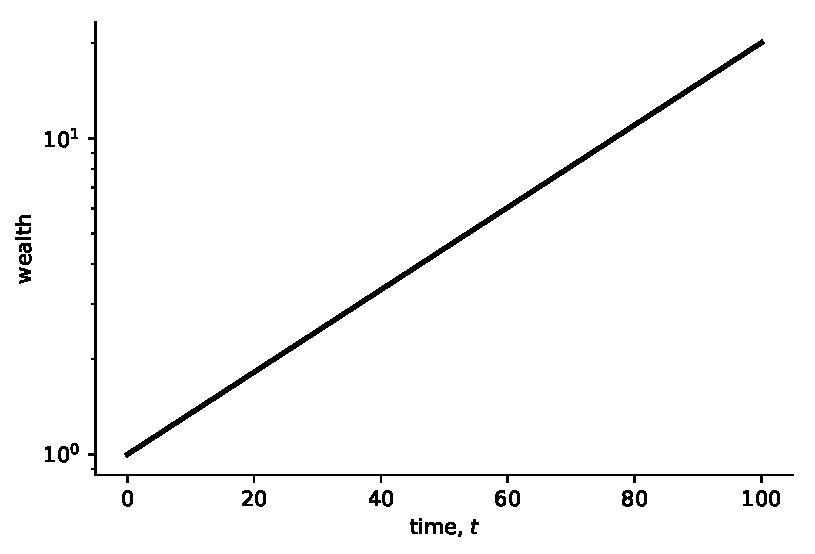
\includegraphics[width=.47\textwidth]{./chapter_risky/figs/add_noise_exp_growth_a.pdf}}
% \put(110,0){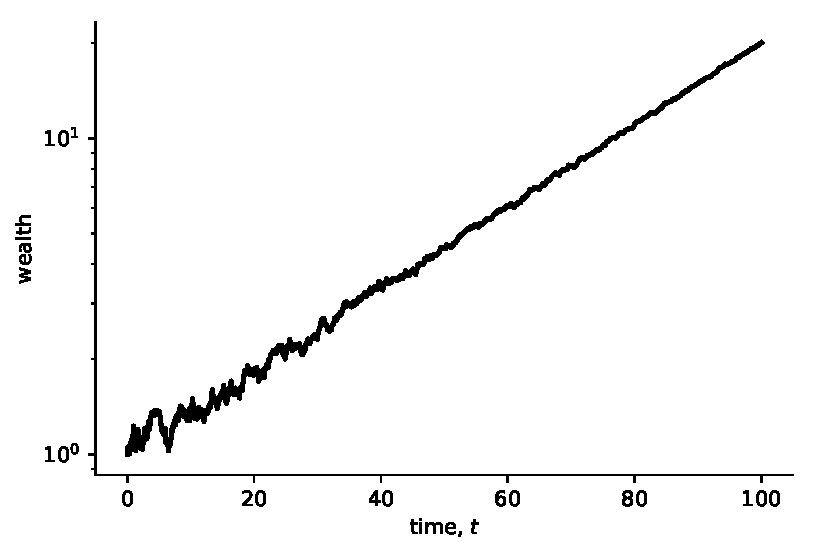
\includegraphics[width=.47\textwidth]{./chapter_risky/figs/add_noise_exp_growth_b.pdf}}
%\end{picture}
%\caption{\small {\bf Left} Exponential growth at 0.03 per time unit. {\bf Right} as left, but we've added a constant-amplitude perturbation to the process.
%As $x$ grows, the perturbation becomes insignificant relative to $x$.}
%\flabel{u_of_x}
%\end{figure}
%
%Of course we're free to model wealth in any way we like. 
%
%
%Our model rationale for deciding between two gambles is simple: 
%given a model for the mode of repetition, 
%choose the gamble with the largest time-average growth rate. 
%In other words, choose the gamble which, 
%if repeated indefinitely, causes your wealth to grow fastest.
%
%We are not saying that real repetitions are necessary. We 
%merely create model humans who base decisions on what would 
%happen to their wealth if they were repeated (infinitely many times). It is a 
%conceptual device -- in effect a thought experiment -- to elicit the 
%underlying tendency of each gamble. A particular choice that can be 
%represented by gambles 
%may be offered only once and, indeed, in the real world this will 
%often be the case. However, in the real world it is also the case 
%that a decision is likely to be followed by many others, a scenario 
%to which indefinite repetition is a plausible approximation.
%
%In our thought experiment this decision rule outperforms any other 
%decision rule almost surely: so, at least in that imagined world, the 
%rationale has a physical basis. If our thought experiment is a good 
%approximation to real-world decision scenarios, then our rationale 
%should be a good model of real-world decisions. Certainly it is 
%parsimonious, based on a single, 
%robust quantity and requiring only the gamble and its mode of repetition 
%to be specified. Unlike some treatments of human decision-making, it 
%contains no arbitrary or hard-to-measure psychological factors.
%
%Having said all this, while we think that the decision axiom 
%is reasonable, we stress that at this point it is an \textit{axiom}, \ie something we assert without empirical justification and which is not deduced from more primitive considerations. It 
%defines a model world where certain types of behaviour will be observed. 
%We will show in \secref{Copenhagen} and in \cref{Markets} why we feel reminded 
%of reality by this model world, though you may disagree 
%and you may prefer a different model that creates a different model world
%that reminds you more of reality.
%Other decision axioms are 
%possible and, indeed, have been proposed. For instance, 
%classical decision theory is defined by the axiom that decision
%makers maximize expected utility -- though \secref{Copenhagen} 
%shows that this model has flaws that may not be acceptable. 
%
%%Copenhagen experiment? Little excursion?
%
%Our decision rationale can be expressed as a set of instructions.
%We denote quantities relating to the $\m^\text{th}$ available gamble with the 
%superscript $(\m)$. Each gamble is specified by its random payout, $\Q^{(\m)}$, and 
%per-round period, $\dt^{(\m)}$. 
%
%\begin{keypts}{Growth-optimal decision algorithm}
%\begin{enumerate}
%\item Specify $\Q^{(\m)}$ and $\dt^{(\m)}$ for the gambles offered;
%\item Specify the wealth dynamic, \ie the relationship between $\d\x(\t)$, 
%$\x(\t)$, and $\q$;
%\item Find the ergodicity transformation, $\gv(\x)$, of the wealth whose increments are 
%instances of a (time-independent) random variable under this dynamic;
%\item Determine the time-average growth rates, $\gt^{(\m)}$, either by taking 
%the long-time limit of the growth rates, $\g^{(\m)}(\t,\Dt)$, or by invoking the 
%ergodic property and taking their ensemble averages;
%\item Choose the gamble, $\m$, with the largest time-average growth rate.
%\end{enumerate}
%\end{keypts}
%
%In examples, we will focus on choices between two 
%gambles, \ie $\m\in\{1,2\}$. Decisions between three or more gambles 
%are straightforward extensions.
%Often one of the gambles presented is the null gamble, which trivially 
%has a growth rate of zero. In this case, the question is 
%whether the other gamble is preferable to doing nothing, 
%\ie bet or no bet?

%We will illustrate the decision algorithm by applying it to the coin toss 
%game of \cref{Coins}. $\x(\tn)>\$ 0$ is the starting 
%wealth and $\dt$ is the time between rounds for each of the 
%gambles offered. We recall that the coin toss gamble is specified by the random payout:
%\bea
%\q^{(1)}_1 = -0.4\x(\tn), &\quad& \p^{(1)}_1 = 1/2; \\
%\q^{(1)}_2 = 0.5\x(\tn), &\quad& \p^{(1)}_2 = 1/2.
%\eea
%Note that, in our setup, the payouts $\Q^{(\m)}_\gi$ are always fixed 
%monetary amounts. Here they are expressed as fractions of $\x(\tn)$, 
%which is itself a fixed monetary wealth.\footnote{Even though this 
%formulation might appear to encode a multiplicative dynamic (largely 
%because it comes from an imagined multiplicative game), we have 
%arranged things so that formally it does not. Indeed, it encodes no 
%dynamic at all: that is specified separately.} We shall ask our individual 
%to choose between the coin toss and the null gamble,
%\be
%\q^{(2)}_1 = \$0, \quad \p^{(2)}_1 = 1.
%\ee
%Both the additive and multiplicative versions of the repeated gamble are analysed.
%
%\begin{example}{Additive coin toss game}
%If the repetition is additive, wealth will evolve over $T$ rounds according to:
%\bea
%\x^{(1)}(t_0+\T\dt) &=& \x(\tn) + \sum_{\gtau=1}^\T \q^{(1)}(\gtau); \\
%\x^{(2)}(t_0+\T\dt) &=& \x(\tn).
%\eea
%Here we have assumed that wealth is free to go negative, \ie that 
%there is no bankrupt state from which the individual can't 
%recover.\footnotemark\ The ergodicity transformation is the identity, 
%$\gv(\x)=\x$, so the growth rates are simply the rates of change of 
%wealth itself. We can express these over the $\T$ rounds as:
%\bea
%\gad^{(1)}(\t) = \frac{\x^{(1)}(\t+\T\dt) - \x(\tn)}{\T\dt} &=& \frac{1}{\T}\sum_{\gtau=1}^\T \frac{\q^{(1)}(\gtau)}{\dt}; \elabel{g1_add}\\
%\gad^{(2)}(\t) = \frac{\x^{(2)}(\t+\T\dt) - \x(\tn)}{\T\dt} &=& \$ 0
%\eea
%per unit time. The long-time limit of the growth rate for the null gamble 
%is trivially $\gad^{(2)}=\$0$ per unit time. For the coin toss, we calculate it as
%\bea
%\overline{\gad}^{(1)} &=& \lim_{\T\to\infty}\left\{\frac{1}{\T}\sum_{\gtau=1}^\T \frac{\q^{(1)}(\gtau)}{\dt}\right\}\\
%&=& \ave{\frac{\q^{(1)}}{\dt}}\\
%&=& \frac{\p^{(1)}_1 \q^{(1)}_1 + \p^{(1)}_2 \q^{(1)}_2}{\dt}\\
%&=& \frac{0.05\x(\tn)}{\dt},
%\eea
%which is positive (assuming $\x(\tn)>\$0$). Therefore, $\overline{\gad}^{(1)}>\overline{\gad}^{(2)}$ 
%and our individual should accept the coin toss gamble under additive dynamics.
%\end{example}
%\footnotetext{We could model this realistic feature by an absorbing boundary on $\x(\t)$, if we were so minded.}
%
%We see from this example that the decision rule under additive repetition is to 
%maximise $\ave{\q/\dt}$.\footnote{Too frequently in presentations of decision 
%theory, it is assumed implicitly that $\dt$ is the same for all available gambles 
%and the decision algorithm is presented as the maximisation of the expected 
%payout, $\ave{\q}$. While this is equivalent if all the $\dt^{(\m)}$ are identical, it 
%is not if they aren't. Moreover, the assumption is usually left unstated. This is 
%unhelpful in that it masks the important role of time in the analysis and, in 
%particular, the fact that our individual is maximising a \textit{rate}.} This is the 
%rate of change of the expected wealth, which, as we know from \eref{g_bar_a}, 
%happens to coincide under this dynamic with the time-average growth rate. We 
%will see later that humans tend not to act to maximise $\ave{\q/\dt}$ in reality. 
%This may not be a great shock: additive repetition without bankruptcy isn't 
%going to win many prizes for the most realistic model of wealth evolution.
%
%Let's try multiplicative repetition instead.
%
%\begin{example}{Multiplicative coin toss game}
%The payout, $\Q^{(1)}$, is re-expressed as a per-round multiplier,
%\be
%\gr^{(1)} = \frac{\x(\tn)+\q^{(1)}}{\x(\tn)},
%\ee
%which takes the values:
%\bea
%\gr^{(1)}_1 = \frac{\x(\tn)+\q^{(1)}_1}{\x(\tn)} = 0.6, &\quad& \p^{(1)}_1 = 1/2; \\
%\gr^{(1)}_2 = \frac{\x(\tn)+\q^{(1)}_2}{\x(\tn)} = 1.5, &\quad& \p^{(1)}_2 = 1/2.
%\eea
%Under multiplicative dynamics, the wealth evolves according to:
%\bea
%\x^{(1)}(\tn+\T\dt) &=& \x(\tn) \prod_{\gtau=1}^\T \gr^{(1)}(\gtau); \elabel{W1T_mult}\\
%\x^{(2)}(\tn+\T\dt) &=& \x(\tn).\elabel{W2T_mult}
%\eea
%The ergodicity transformation is the logarithm, $\gv(\x)=\ln \x$. We have 
%already discussed why, but one way of seeing this is to take logarithms of 
%\eref{W1T_mult}. This converts the product into a sum of independent instances of a random variable:
%\bea
%\ln \x^{(1)}(\tn+\T\dt) &=& \ln \x(\tn) + \sum_{\gtau=1}^\T \ln \gr^{(1)}(\gtau); \elabel{lnW1T_mult}\\
%\ln \x^{(2)}(\tn+\T\dt) &=& \ln \x(\tn).\elabel{lnW2T_mult}
%\eea
%Therefore, $\ln \x$ is the desired quantity whose increments 
%inherit their ergodicity from $\q$. The growth rates, expressed over $\T$ rounds, are:
%\bea
%\gm^{(1)}(\t) = \frac{\ln \x^{(1)}(\t+\T\dt) - \ln \x(\tn)}{\T\dt} &=& \frac{1}{\T}\sum_{\gtau=1}^\T \frac{\ln \gr^{(1)}(\gtau)}{\dt};\\
%\gm^{(2)}(\t) = \frac{\ln \x^{(2)}(\t+T\dt) - \ln \x(\tn)}{\T\dt} &=& 0
%\eea
%per unit time. As in the additive case, we take the $\T\to\infty$ limits. For the null 
%gamble this is trivial: $\gt_\text{m}^{(2)}=0$ per unit time. For the coin toss gamble, we get
%\bea
%\gt_\text{m}^{(1)} = \ave{\frac{\ln \gr^{(1)}}{\dt}} = \frac{\ln\left(\sqrt{0.9}\right)}{\dt},
%\eea
%which is negative. Thus, $\overline{\gm}^{(1)}<\overline{\gm}^{(2)}$ under multiplicative 
%dynamics and our individual should decline the coin toss. That this is the opposite 
%of his decision under additive repetition highlights the importance of specifying a 
%dynamic that corresponds well to what is happening in reality.
%
%Another way of presenting the repeated coin toss is to express the wealth 
%after $\T$ rounds as
%\be
%\x^{(1)}(\tn+\T\dt) = \x(\tn)\left(\gr_\T^{(1)}\right)^\T,
%\ee
%where
%\be
%\gr_\T^{(1)} = (0.6)^{(\T-\gk)/\T}(1.5)^{\gk/\T}
%\ee
%is the equivalent per-round multiplier after $\T$ rounds and 
%$0\leq \gk\leq \T$ is the number of winning rounds. $\gr_\T$ 
%is a random variable but it converges almost surely to a scalar in the long time limit,
%\be
%\gr_\infty^{(1)} \equiv \lim_{\T\to\infty}\{\gr_\T^{(1)}\} = (0.6)^{1/2}(1.5)^{1/2} = \sqrt{0.9},
%\ee
%since $\gk/\T\to1/2$ as $\T\to\infty$ (the coin is fair). $\gr_\infty^{(1)}<1$ so the 
%individual's wealth is sure to decay over time and he should decline the gamble. 
%The two approaches are, of course, linked, in that
%\be
%\gt_\text{m}^{(1)} = \frac{\ln \gr_\infty^{(1)}}{\dt}.
%\ee
%\end{example}
%
%Here we see that our decision rule boils down to maximising
%\be
%\ave{\frac{\ln \gr}{\dt}} = \ave{\frac{\ln(\x(\tn)+\q)-\ln \x(\tn)}{\dt}}.
%\ee
%This coincides with the time-average growth rate in \eref{g_bar_m}.
%
%===============================================

\section{Relation to earlier economic theories \seclabel{Relation_to_earlier}}
In the previous section we presented the ergodicity economics model of decision-making: maximise the time-average growth rate of wealth.
That's it; everything in ergodicity economics can be related back to this simple idea. 

In the present section, we will detail precisely how our model is related to models that were developed earlier, 
specifically at a time before the ergodicity question had been asked. This section is thus about history: how did we
model human decision making under risk before we knew we had to find appropriate growth rates?

The story is fascinating: despite the absence of appropriate tools and concepts, early researchers
invented ingenious mathematical representations of human behaviour. With not very much work, it is 
possible to tweak these models, at least in special cases, to coincide with ergodicity economics.

The roadmap for this section is as follows. We will first introduce the concept of a {\it gamble} -- in essence that's a 
little piece of a stochastic process, a random wealth change realised over some short time. Next, we will 
mention the {\it gamble problem}, namely the problem of choosing between different gambles when we have 
to. To connect to ergodicity economics, we point out how different ways of repeating a gamble 
can generate different dynamics, very similar to the types considered in \secref{Perturbing}.
Finally, we will present the classic solution to the gamble problem, which assigns a utility $\gu(\x)$ -- non-linear in wealth -- to
monetary wealth. This will be summarised in the expected-utility-theory decision algorithm.

%Conversely, putting many gambles in a row can generate a wealth trajectory, just like our perturbed wealth dynamics.
%The really fascinating bit is called expected utility theory: as early as 1738 -- long before the ergodicity debate -- 
%Daniel Bernoulli noticed that people's behaviour is often quite well modelled as optimizing the expectation value 
%of changes in the logarithm of wealth. We already know what that means: it corresponds to people optimising 
%the time-average growth rate under multiplicative dynamics. But Bernoulli didn't have those concepts at his 
%disposal, and simply stated that people have what he called a ``utility function,'' namely a non-linear transformation 
%of wealth whose expected changes they optimise. We already know this transformation: it's the ergodicity mapping 
%that allows us to compute time-average growth rates as expectation values. Bernoulli called the function 
%$\gu(\x)$, we called it $\gv(\x)$. Of course the function can be the same, \eg the logarithm. But its the meaning 
%of $\gu$ is very different from the meaning of $\gv$. The former, supposedly, is a property of a person -- it 
%describes someone's character. The latter, $\gv$, is not a property of a person but a property 
%of a dynamic. It doesn't matter whose wealth is subjected the dynamic with ergodicity transformation 
%$\gv$ -- if it's $\gv$, that's what's being optimised under EE.

\subsection{Gamble: random number and duration}
\seclabel{Gamble:}
One fundamental building block of mathematical decision theory is the gamble.
This is a mathematical object that resembles a number of situations in real life, 
namely situations where we face a decision whose consequences will be purely
financial and are somewhat uncertain when we make the decision. An 
example is buying a lottery ticket. We define the gamble mathematically as follows.

\begin{defn}{Gamble}
A gamble is a pair of a random variable, $\Q$, and a duration,  $\dt$. 
\vspace{.2cm}

$\Q$ is called the payout and takes one of $\K$ (mutually exclusive) possible monetary 
values, 
$\{\q_1,\ldots,\q_{\K}\}$, associated with probabilities, $\{\p_1,\ldots,\p_{\K}\}$, where 
$\sum_{\gj=1}^\K \p_\gj = 1$. 
Payouts can be positive, associated with a monetary gain, or negative, 
associated with a loss. We order them such that $\q_1<\ldots<\q_\K$.
\end{defn}

%Everything we need to know about the gamble is contained in the payouts, probabilities, and duration. 
In economics, the duration of a gamble is rarely discussed but it's clearly crucial information, as a trivial example shows. Let's say you get to choose between two gambles. One pays $\$1$ with probability $1$ and takes one second to complete; the other also pays $\$1$ also with probability $1$ but takes one year to complete. Clearly the former is more attractive. Knowing the duration will also be necessary to relate the gamble to ergodicity economics -- the latter being based on time, this should come as no surprise.

The following situations may be modelled as gambles:

\begin{example}{Betting on a fair coin}
Imagine betting $\$ 10$ on the toss of a fair coin. We would model this 
with the following payouts and probabilities:
\bea
\q_1 = -\$ 10, &\quad& \p_1 = 1/2;\\
\q_2 = +\$ 10, &\quad& \p_2 = 1/2.
\eea
The duration may be the time until you receive the payout, or if you participate in one coin toss every week, say, we may want to make it $\dt=1$ week.
\end{example}

\begin{example}{Playing the lottery}
We can also imagine a gamble akin to a lottery, where we pay an amount, 
$\F$, for a ticket which will win the jackpot, $\J$, with probability, $\p$. The corresponding 
payouts and probabilities are:
\bea
\q_1 = -\F,  &\quad& \p_1 = 1-\p;\\
\q_2 = \J-\F, &\quad& \p_2 = \p.
\eea
Note that we deduct the ticket price, $\F$, in the payout $\q_2$.
The duration may be $\dt=1$ week.
\end{example}

%\begin{example}{Betting at fixed odds}
%A bet placed at fixed odds, for example on a horse race can also be modelled as a gamble. 
%Suppose we bet on the horse \textit{Ito} to win the 2015 Prix de l'Arc de Triomphe 
%in Paris at odds of 50/1 (the best available odds on 20th September 2015). 
%\textit{Ito} will win the race with unknown probability, $\p$. If we bet $\F$, 
%then this is modelled by payouts and probabilities:
%\bea
%\q_1 = -\F,  &\quad& \p_1 = 1-\p;\\
%\q_2 = 50\F, &\quad& \p_2 = \p.
%\eea
%The duration may be something like $\dt=30$ minutes.
%\end{example}

\begin{example}{The null gamble}
It is useful to introduce the null gamble, in which a payout of zero is received 
with certainty: $\q_1=\$0$, $\p_1=1$. This represents the `no bet' or `do nothing' option.

As in the examples above, the duration, $\dt$, has to be chosen appropriately. 
The meaning of the duration will become clearer later on -- often it is the time 
between two successive rounds of a gamble.
\end{example}

%The gamble is a simple but versatile mathematical model of an uncertain future. 
%It can be used to model not only traditional wagers, such as sports bets and 
%lotteries, but also a wide range of economic activities, such as stock market 
%investments, insurance contracts, derivatives, and so on. 
The gamble we have 
presented is discrete, in that the payout, $\Q$, is a random variable with a 
countable (and, we usually assume, small) number of possible values. 
The extension to continuous random variables is natural and used frequently 
to model real-world scenarios where the number of possible outcomes, \eg the change 
in a stock price over one day, is large.

This presents a natural connection to ergodicity economics: given a stochastic wealth 
process $\gd\x$, the wealth change generated by that process over a certain time 
interval $[\t,\t+\dt]$ is a gamble. The random variable is 
\be
\Q=\int_\t^{\t+\dt} \gd\x,
\elabel{gamble_from_process}
\ee and the duration is $\dt$.

Suppose now that you have to choose between two options that you've modelled 
as two gambles (possibly including the null gamble). Which should you choose, 
and why? This is the gamble problem, the central question of decision theory, and 
the basis for much of mainstream economics.

\begin{defn}{The gamble problem}
The gamble problem is the problem to choose between two gambles.
\end{defn}

We stress here that the gamble alone is not enough information to answer this question. 
The value of a gamble -- clearly -- depends on more facts than probabilities, payouts, and duration. Crucially, it depends on 
\begin{enumerate}
\item
how the gamble affects our future. For instance: if we go bankrupt as a result, can we recover from that?
\item
our circumstances. When you're very rich you can afford to take risks that you can't afford when you're poor. 
\item
our personality. Some like the thrill of gambling, others find it unpleasant.
\end{enumerate}
Mainstream economics focuses on point 3. Ergodicity economics, on the other hand, focuses on points 1 and 2, 
where we would compute the average growth rates of the processes corresponding to the gambles. 
Even in the simple case of multiplicative dynamics, this requires knowledge of the individual's wealth 
before the gamble, $\x(\t)$. It also requires knowledge of the process itself. Without that we wouldn't 
know the form of the ergodic growth rate; we wouldn't know what to compute. 

Although the gamble problem is underspecified by gambles alone, the gamble is a 
useful conceptual unit because it specifies that part of the model of evolving wealth 
that is independent of individual circumstances. It thus splits an easily observable part
of the problem from information that's much harder to obtain. We can all buy the same 
lottery ticket with publicly specified prizes, probabilities, duration -- for some of us that 
will be attractive, for others it won't, for a variety of reasons.

%%%%%%%%%%%%%%%%%%%%%%%%%%%%%%%%%%%%%%%%%%%%%%%
\subsection{Repeated gamble: towards a wealth process}
\seclabel{Repeated_gamble}

We already know one touch point between ergodicity economics and 
the classic gamble setup: we know how to construct a gamble as the random variable 
corresponding to a time interval of a stochastic process -- that's \eref{gamble_from_process}.
Ergodicity economics specifies how to evaluate a wealth process, and if
it's justifiable to identify the gamble with the process, then we know how to evaluate 
the gamble under ergodicity economics. 
%we must propose a criterion to choose between two
%gambles. Different criteria will result in different decisions -- by writing down a criterion
%we build a model world of model humans who behave in ways that may seem sensible
%to us or crazy -- if the behaviour seems crazy we have probably not chosen a good
%criterion and we should look back, think about what may be wrong with the criterion, 
%and try a better one.

We will now strengthen this connection by showing what it might mean to identify the gamble 
and the process. To do this we will take a gamble and construct from it a 
wealth process. That means we have to extend the gamble over an arbitrarily long time. 
A principled way of doing that (one that keeps extra assumptions to a minimum and clearly visible)
is to imagine the gamble is being repeated over and over again. 

%The wealth process $\x(\t)$ is related to the gambles our model humans 
%choose to play. Precisely {\it how} it is related remains to be specified.
%
%Considering a single round of a gamble in isolation -- the so-called `one-shot' setup 
%-- is relatively uninstructive in this regard, though that hasn't diminished its prominence in wider literature. 
%All we know is 
%that one of the possible payouts will be received, leading to the random value 
%$\x(\t+\dt)=\x(\t)+\q$. 
%We don't yet know how accepting this gamble will affect how our wealth, $\x(\t)$, grows or decays over time, since one time step isn't enough for this to become apparent. 
%The one-shot game takes one random value, $\q$, and turns it trivially into 
%another, $\x(\t)+\q$. Time has no significance in a 
%one-shot game. An amount $\dt$ elapses, but this could be a single 
%heartbeat or the lifetime of the universe, for all the difference it makes to the analysis.
%
%To establish how your wealth evolves, we must imagine that the world does 
%not come to a grinding halt after the gamble. Instead we imagine that the gamble
%is repeated over many rounds.\footnote{In fact, to make the 
%problem tractable mathematically, it will be necessary to imagine the gamble 
%is repeated indefinitely.} This does not mean that we actually
%believe that a real-world situation will repeat itself over and over again, \eg we don't
%believe that we will bet on the horse \textit{Ito} at odds 50/1 many times in a row. Instead, 
%imagining repetition is a methodological device that allows us to extract tendencies
%where they would otherwise be invisible. It is the model analogue of 
%the idea that individuals live in time and that their decisions have consequences 
%which unfold over time.

Crucially, {\it the mode of repetition is not specified in the gamble itself.} It is the only
additional assumption we have to make to arrive at a wealth process and unlock the 
power of ergodicity economics. We shall 
focus on two modes: \textit{additive} and \textit{multiplicative} repetition, which
correspond to additive and multiplicative dynamics. Thus {\it the same gamble can 
correspond to different dynamics.}
%Other dynamics will be considered later on, in \secref{general_dynamics}.

\subsubsection{Additive repetition}
\begin{defn}{Additive repetition}
If a gamble is repeated additively, then a newly generated realization of the random 
payout, $\q$, is added to $\x(\t)$ in each round. We define the change in wealth 
occurring over a single round as
\be
\d \x(\t) \equiv \x(\t+\dt)-\x(\t).
\elabel{DW_def}
\ee
In the additive case, we have
\be
\d\x(\t) = \q.
\elabel{DW_add}
\ee
In other words, under additive repetition, $\d \x$ is a stationary 
random variable, meaning the ergodicity transformation is the identity, 
$\gv(\x)=\x$, and we're in the case of additive dynamics.
%\footnote{This seemingly mundane corollary stems 
%from our definitions of $\gD$ as a monetary payout and $\d\x$ as an 
%additive change in wealth, expressed in monetary units. It would not 
%hold if, for example, we had defined $\d\x$ to be some other type of 
%change, such as a relative change.}
Starting at time, $\tn$, wealth 
after $\T$ rounds is
\be
\x(\tn+\T\dt) = \x(\tn) + \sum_{\gtau=1}^\T \q(\gtau),
\elabel{Wt_add}
\ee
where $\q(\gtau)$ is the realisation of the random variable in round $\gtau$. 
This is an evolution equation for wealth following a noisy additive dynamic. 
Note that $\x(\tn+\T\dt)$ is itself a random variable.
\end{defn}


\begin{example}{Additive repetition of a \$10 bet}
We return to our first example of a gamble: a $\$ 10$ bet on 
a coin toss. Under additive repetition, successive bets will always 
be $\$ 10$, regardless of how rich or poor you 
become. Suppose your starting wealth is $\x(\tn)=\$ 100$. 
Then, following \eref{Wt_add}, your wealth after $\T$ rounds will be
\bea
\x(\tn+\T\dt) &=& \$ 100 + \$ 10 \gk - \$ 10 (\T-\gk)\\
&=& \$ [100 +  10(2\gk-\T)],
\eea
where $0\leq \gk\leq \T$ is the number of tosses you've won. Note that
we have assumed your wealth is allowed to go negative. If not, then the 
process would stop when $\x<\$ 10$, since you would be unable 
to place the next $\$ 10$ bet.
\end{example}

\subsubsection{Multiplicative repetition}
An alternative is multiplicative repetition. In the example above, let 
us imagine that the first $\$ 10$ bet were viewed not as a bet 
of fixed monetary size, but as a fixed fraction of the 
starting wealth ($\$ 100$). Under multiplicative repetition, each 
successive bet is for the same fraction of wealth which, 
in general, will be a different monetary amount.

The formalism is as follows. 
\begin{defn}{Mulitplicative repetition}

The payout, $\q_{\gj}$, in the first round is 
expressed as a random wealth multiplier,
\be
\gr_{\gj} \equiv \frac{\x(\tn)+\q_{\gj}}{\x(\tn)}.
\elabel{R_def}
\ee
This multiplier is another random variable, and multiplicative repetition 
means drawing a new instance of it every $\dt$ and multiplying wealth 
$\x(\t)$ accordingly.
% -- it also (trivially) 
%defines a stochastic process that is a new instance of the 
%random variable at each point in time, $\gr(\t)$. The gamble 
%is repeated by applying another instance of the same 
%multiplier at all subsequent rounds:
%\be
%\x(\t+\dt) = \gr(\t)\x(\t).
%\ee
%In each round of the gamble, 
Wealth after $\T$ rounds of the multiplicatively repeated gamble is
\be
\x(\tn+\T\dt) = \x(\tn)\prod_{\gtau=1}^\T \gr(\gtau),
\ee
where $\gr(\gtau)$ is the realisation of the random multiplier in round $\gtau$.
%From \eref{R_def} we see that $\gr(\t)$ is a sequence of instances 
%of a random variable with time-independent distribution, 
%since it depends only on $\Q$, which is time-independent, and the starting 
%wealth, $\x(\tn)$, which is fixed. However, distributions of successive changes in wealth,
%\be
%\d \x(\t) = (\gr-1)\x(\t),
%\elabel{DW_mult_short}
%\ee
%are not time-independent, as they depend on $\t$ through $\x(\t)$. 
The ergodicity transformation is now $\gv(\x)=\ln\x$, by which we mean that logarithmic wealth 
changes, $\d\ln\x$, are stationary. The exponential growth rate is ergodic, and its expectation value
\be
\frac{\ave{\d\ln\x}}{\dt}
\ee
is the time-average growth rate under this mode of repetition.
\end{defn}

\begin{example}{Multiplicative repetition}
The $\$10$ bet on a coin toss is now re-expressed as a bet of a fixed 
fraction of wealth at the start of each round. Following 
\eref{R_def}, the random multiplier, $\gr$, has two possible outcomes:
\bea
\gr_1 = \frac{\$100 - \$10}{\$100} = 0.9, &\quad& \p_1 = 1/2;\\
\gr_2 = \frac{\$100 + \$10}{\$100} = 1.1, &\quad& \p_2 = 1/2.
\eea
The wealth after $\T$ rounds is, therefore,
\be
\x(\tn+\T\dt) = \$100\,\,(1.1)^\gk\,(0.9)^{\T-\gk},
\ee
where $0\leq \gk \leq \T$ is the number of winning tosses. In this example there is 
no need to invoke a `no bankruptcy' condition, since we can lose no 
more than 10\% of our wealth in each round.
\end{example}

%The difference between the two modes of repetition might easily be mistaken 
%for a matter of taste. When the $\$ 10$ bet was first offered, what 
%difference does it make whether our individual imagined this to be a bet of a 
%fixed size or of a fixed fraction of his wealth? However, the consequences of 
%this choice between imagined situations are enormous, as we shall see 
%experimentally in \secref{Copenhagen}. In \cref{Coins} we saw that additive and multiplicative dynamics differ as starkly as the 
%linear and exponential functions, and there is evidence that people adjust their behaviour
%to the type of repetition they face. 
%%CPH
%It matters, therefore, that we consider 
%carefully the economic situation we wish to model in order to choose the 
%most realistic mode of repetition. For example, fluctuations in the price of a 
%stock tend to be proportional to the price, \cf \eref{DW_mult_short}, so 
%multiplicativity is the appropriate paradigm for large wealth fully invested in stocks.

%Now that we've established how the gamble is related to $\x(\t)$ we can 
%begin to think about decision criteria. Not surprisingly, appropriate
%growth rates are useful decision criteria -- ``pick the gamble that will make
%your wealth grow fastest'' is generally good advice. To be able to 
%follow this advice we will think again about growth rates.
We have defined a gamble and clarified how it is related to ergodicity economics. 
It can be derived from a wealth dynamic; conversely a wealth dynamic can be 
constructed from a gamble provided we know 
how to repeat the gamble. But early decision theory didn't use the concepts of 
repetition, time averages, or ergodicity transformations. In the next section we will 
present how the gamble problem was addressed before the advent of ergodicity 
economics, and precisely how this earlier treatment is related to ours.

%%%%%%%%%%%%%%%%%%%%%%%%%%%%%%%%%%%%%%%%%%%%%%%
%\subsection{Expected utility theory}
%\seclabel{Expected_utility}
%%%%%%%%%%%%%%%%%%%%%%%%%%%%%%%%%%%%%%%%%%%%%%%
\subsection{Expected wealth and expected utility}

In ergodicity economics, we solve the gamble problem by maximizing the time 
(or ensemble) average of the ergodic growth rate for the process we consider 
the gamble to be part of. 

But until recently, this was not how economists treated the gamble problem. It's instructive
to mention two earlier criteria for gamble evaluation: the expected wealth change, 
invented around 1654; and the expected utility change, invented around 1738. Despite the 
conceptual error embedded in these criteria -- confusing expectation values with time 
averages -- they are easy to express in terms of time averages and ergodicity economics. 
In later developments, such as extensions of expected-utility theory beginning in the 1930s, 
and of prospect theory in the 1970s, the original error is compounded, and it is unclear 
how to ascribe physical meaning to the resulting models.


%
%Our decision rule under additive repetition of the gamble is to maximise
%\be
%\ave{\frac{\d\x}{\dt}} = \ave{\frac{\q}{\dt}},
%\elabel{ex_crit}
%\ee
%\ie the rate of change of the expectation value of wealth. This was, in fact, 
\subsubsection{Expected wealth}
The first gamble evaluation criterion, which emerged in the early 
days of probability theory in the $17^\text{th}$ century, was this:

\begin{keypts}{Expected wealth decision algorithm}
\begin{enumerate}
\item Specify $\Q^{(\m)}$ for the gambles offered;
\item Determine the change of expected wealth induced by each gamble,
\be
\ave{\d\x}^{(m)}=\ave{\Q{(^m)}};
\elabel{EUT_criterion}
\ee
\item Choose the gamble, $\m^*$, with the largest $\ave{\d\x}^{(\m)}$.
\end{enumerate}
\end{keypts}

The history of this criterion is linked to finding what was perceived as a fair value
of an uncertain prospect. Say we're playing a game of chance, for some amount of 
money in a pot, maybe we're rolling dice, best out of three. If you're currently ahead, 
say after two throws, and someone wants to take over your 
position, it may be fair to sell your position for the expectation value of your 
winnings. One reason this criterion makes some sense is conservation: the sum 
of the expected winnings of all players is precisely the pot, so buying everyone 
out of his position is equivalent to buying the pot, as perhaps it should be.

Connecting this back to ergodicity economics: under what conditions would we evaluate a gamble 
by computing $\ave{\d\x}$? 
%Strictly: never -- we really need to know the duration of the gamble, $\dt$.
%This duration is rarely mentioned in the early gambling texts, a first hint that considerations of time
%did not dominate the thinking in this space. But it's just a hint, not a major stumbling block: 
%if $\dt$ is the same for all gambles -- whatever the dynamic -- it will cancel out when we compare 
%time-average growth rates of different gambles.
The answer is: under additive dynamics.
The ergodicity economics maximand is then $\ave{\gad}=\frac{\ave{\d\x}}{\dt}$. Apart from the 
$\dt$ in the denominator (which cancels if we assume it's the same for all considered gambles), 
this is expected-wealth maximisation. We conclude that 
expected-wealth maximisation is equivalent to ergodicity economics under the assumption 
of additive wealth dynamics: one of the simplest wealth models we can write down.

There is even a good reason why additive dynamics may have been 
assumed in the early developments. Let's Taylor-expand the time average of the general 
ergodic growth rate (which we may write as an ensemble average because of ergodicity)
\bea
\ave{\g}&=&\frac{\ave{\d\gv(\x)}}{\dt}\\
&=&\frac{1}{\dt} \ave{\left[\frac{\gd\gv}{\gd\x}\d\x+\frac{1}{2}\frac{\gd^2\gv}{\gd\x^2}\d\x^2 + \cdots \right]}\\
&=&\frac{1}{\dt} \left[\frac{\gd\gv}{\gd\x}\ave{\d\x}+\frac{1}{2}\frac{\gd^2\gv}{\gd\x^2}\ave{\d\x^2} + \cdots \right]
\eea
The last line follows from the fact that the derivatives of $\gv$ are known functions, evaluated at the
known wealth $\x$ before the gamble takes place. In other words, they are just constants and can be
taken out of the expectation operator, $\ave{\cdot}$.
If $\d\x$ is small, keeping only the first term in the expansion is often a valid approximation, in 
which case we will call the dynamic ``linearisable,'' and the expression becomes
\be
\approx \frac{\ave{\d\x}}{\dt} \frac{\gd\gv}{\gd\x},
\ee
which is proportional to the expected wealth change. In behavioural terms, being 
proportional means yielding the same ranking of any set of gambles as just the expected wealth $\ave{\d\x}$.

{\bf Summary:} the first formal decision theory is expected wealth maximization. This theory is equivalent to ergodicity economics under additive dynamics, and additive dynamics are equivalent to any linearisable dynamic in the small-stakes limit.

\subsubsection{Expected utility}
%
%. We will call this the 
%`expected-wealth paradigm'. It was not derived as we have derived it, from a 
%criterion to maximise growth over repetition. Instead, it was essentially proposed 
%as the decision axiom itself, with no reference to dynamics. It is easy to see why: 
%it is a simple rule containing a familiar type of average, which incorporates all the 
%possible outcomes of the game. Indeed, it would be logically sound if we could play 
%the game many times in parallel, thereby accessing all the possible outcomes.
%
In the language of economics, the expected-wealth paradigm treats humans as 
`risk neutral', \ie they have no preference between gambles whose expected 
changes in wealth are identical (over the same time interval). For example, 
people would be indifferent to either keeping what they have (the null gamble), or tossing a coin to 
win or lose \$1,000.

At least since 
1713~\cite[p.~402]{Montmort1713}, this has been known to be a flawed model. 
Nicolas Bernoulli pointed out that gambles can be constructed -- at least in theory --
whose expected wealth change does not exist. What then, would this criterion mean?
Moreover, expected wealth maximisation does not always  accord 
well with observed behaviour. For instance, anyone who buys an insurance contract
prefers the certain loss of the insurance fee to a random loss
of smaller expectation value. Such a person does not maximise expected wealth, but 
insurance contracts have been signed since Phoenecian times.

In 1738 Daniel Bernoulli put forward a new model of human behaviour that addressed
some of the empirical failures of expected wealth maximisation\footnote{Bernoulli's original paper contains an error. The theory as we present it here is a corrected version that can be found in \cite{Laplace1814}, see also \cite{Peters2019} for a discussion of the error}. 

Bernoulli noted that the value to an 
individual of a possible change in wealth depends on how much wealth the individual already 
has and on his psychological attitude to taking risks. In other words, people do not 
treat equal amounts of extra money equally. This makes intuitive sense: an extra 
$\$10$ is much less significant to a rich man than to a pauper for whom it 
represents a full belly; an inveterate gambler has a different attitude to risking 
$\$100$ on the spin of a roulette wheel than a prudent saver, their wealths 
being equal.

In 1738 Bernoulli~\cite{Bernoulli1738}, after correspondence with Cramer, devised 
the `expected-utility paradigm' to model these considerations. He observed that 
money may not translate linearly into usefulness and assigned to an individual 
an idiosyncratic utility function, $\gu(\x)$, that maps his wealth, $\x$, 
into usefulness, $\gu$. He claimed that this was the true quantity whose expected change,
 $\ave{\d\gu(\x)}$, is maximised in a choice between gambles.

This is the axiom of utility theory. It leads to yet another decision algorithm.
\begin{keypts}{Expected-utility decision algorithm}
\begin{enumerate}
\item Specify $\Q^{(\m)}$ for the gambles offered;
\item Specify the individual's idiosyncratic utility function, $\gu(\x)$, which maps his wealth to his utility;
\item Determine the change of expected utility induced by the gamble,
\be
\ave{\d\gu}=\ave{\gu\left(\x+\q^{(\m)}\right)}-\gu(\x);
\elabel{EUT_criterion}
\ee
\item Choose the gamble, $\m^*$, with the largest $\ave{\d\gu}^{(\m)}$.
\end{enumerate}
\end{keypts}

Let's ask the same question as for the expected-wealth paradigm: under what conditions
would ergodicity economics maximise the quantity in \eref{EUT_criterion}?
The utility function $\gu(\x)$ is defined -- somewhat circularly, as \eg von Neumann and Morgenstern 
pointed out \cite[p.~28]{vonNeumannMorgenstern1944} -- as the object whose expected changes 
are maximised by a person. Under ergodicity economics, what's being maximised is the expected 
(rate of) change of the ergodicity transformation, $\gv(\x)$. 

\begin{keypts}{Mapping: expected-utility theory $\Leftrightarrow$ ergodicity economics}
We conclude that expected-utility theory is 
equivalent to ergodicity economics if gambles of equal duration, $\dt$ are considered
and {\it if the utility function, $\gu$, coincides with the ergodicity transformation $\gv$.}
\end{keypts}

But it gets even better. Bernoulli did not just write down a general function $\gu(\x)$ but argued
that the logarithm is a plausible candidate for this function. People, he claimed, tend to behave
as if they were optimising expected changes in the logarithm of wealth. Quite why that was the case, he didn't know.
We do: using the logarithm as the ergodicity transformation, \ie equating $\gu=\gv$,
we find that Bernoulli's observation can be rephrased: people commonly maximise the time average of the ergodic growth rate under multiplicative dynamics.
That's the second important wealth model we identified!

This is quite an astonishing correspondence, and we believe it is not coincidental. In the 18th 
century, researchers discovered elements of the mathematical structure of ergodicity 
economics. Just by careful observation -- the appropriate mathematical tools had yet to be invented. 
Because mathematical concepts were immature at the time, a nomenclature 
emerged (``utility,'' ``risk preferences'' {\it etc.}) that seems quaint from today's 
conceptual context.

{\bf Summary:} historically, the second formal decision theory is expected utility maximisation. 
This theory is equivalent to ergodicity economics if the utility function is the ergodicity 
transformation. Each dynamic thus has a corresponding growth-optimal utility function. 
The special case treated by Bernoulli in detail -- logarithmic utility -- is equivalent to 
ergodicity economics under multiplicative dynamics. Expected wealth maximisation 
is a special case of expected-utility maximisation, namely using a linear utility function 
(corresponding to ergodicity economics under additive dynamics).

%
%Despite their conceptually different foundations, we note the similarities between the 
%maximands\footnote{The quantities to be maximised.} of our growth-optimal decision 
%theory, \eref{g_bar_gen}, and the expected-utility paradigm, \eref{euh}. Our decision theory
%contains a mapping which transforms wealth into a variable, $\gv$, whose increments are 
%instances of a time-independent random variable. This mapping depends on the wealth dynamic which 
%describes how the gamble is repeated. The expected-utility paradigm contains a function which transforms 
%wealth into usefulness. This is determined by the idiosyncratic risk preferences of 
%the individual. If we identify the ergodicity transformation of the former with the 
%utility transformation of the latter, then the expressions are the same.
%
%But we caution against the conceptual world of expected utility theory. It uses expectation
%values, where they are inappropriate (because decisions of an individual are considered, 
%not of many parallel systems), and it corrects for this error by introducing a non-linear 
%mapping of wealth (the utility function) whose specific form cannot be pinned down 
%convincingly. Finally, because of this conceptual weakness, utility theory is poorly defined. 
%The very first paper on the topic contains two contradictory definitions of expected utility 
%theory \cite{Bernoulli1738}, and over the centuries several others have been added.
%
%Nonetheless, with a few assumptions, expected utility theory as we've
%presented it above is consistent with growth rate optimisation, provided a suitable pair of dynamic and utility function is used. 
%For multiplicative dynamics, the necessary utility function is the logarithm. That this is the most 
%widely used utility function in both theory and practice is a psychological fluke in the classic mindset; from our perspective it indicates that 
%our brains have evolved to produce growth-optimal decisions in a world governed 
%by multiplicative dynamics, \ie where entities produce more of 
%themselves. Incidentally, a common definition of life is ``that which produces more of itself,'' or as Harold Morowitz put it \cite[p.~5]{Morowitz1992} ``Living systems self-replicate, that is, they give rise to organisms like themselves.'' From our perspective, the prevalence of logarithmic utility reflects our evolution in an environment of living things.
%
%Thus we can offer a different reason for the predictive failure of the expected-wealth 
%paradigm. In our framework this corresponds to good decisions under additive 
%repetition, which we claim is generally a poor model of how wealth evolves.\footnote{It 
%would correspond, for example, to the interest payments in your bank account being 
%independent of your balance!} It fails, therefore, because it corresponds to an unrealistic dynamic. 
%
%It's worth being explicit about how our theory differs from expected utility theory. 
%In our model what's stable about human behavior is this: humans optimize wealth over time. Utility theory says humans optimize utility across the ensemble. Given a dynamic, our paradigm predicts human behavior that can be mapped to a predicted utility function. Utility theory believes that behavior, specifically risk preferences, is an idiosyncratic thing: it does not depend on the dynamics but on the individual. This difference (behavior is determined by dynamics vs. behavior is determined by indiosyncrasy) means that in principle we can find out which theory is right. We can change dynamic and see if people change behavior. That would invalidate expected utility theory. We can also take several people and expose them to the same dynamic -- the extent to which they display utility functions that are incompatible with the dynamic would invalidate our theory, insofar as it is interpreted to predict human behavior. Our theory provides the optimal behavioral protocol, in terms of long-term wealth growth, but of course real humans will only optimize long-term wealth growth to a certain degree. Nevertheless, we are happy to report that a Danish group of experimentalists has recently carried out experiments where subjects were exposed to different wealth dynamics, to see whether the utility functions implied by their behavior changed as predicted by our theory. At the time of writing, we're still waiting for the results.
%
%\section{General dynamics}
%\seclabel{general_dynamics}
%Before we come to example applications of decision theory, it is time to discuss 
%dynamics that are neither additive nor multiplicative and their relation to general
%utility functions. 
%
%\subsection{Why discuss general dynamics?}
%What are we trying to achieve with this? First of all, where the time perspective has come
%up in history, \eg \cite{Whitworth1870,Kelly1956}, it was always in the context of multiplicative 
%dynamics, which, as we saw in the previous section, corresponds to logarithmic utility. One 
%persistent criticism from people trained to think in terms of utility has been: what if my utility 
%function is not logarithmic? In other words, the time perspective has seemed overly restrictive 
%to many people.
%
%As a matter of epistemology, we want to be somewhat restrictive. Imagine the opposite: a 
%model that can produce absolutely any behavior. Because it can produce anything, it cannot 
%say ``the reason this happens and not that is X.'' But that's exactly the type of statement we 
%need in order to make sense of the world -- why do some structures exist and not others? 
%Consider a specific case of a universal model: the alphabet, including punctuation. That's all 
%the building blocks you need to tell any story you want, true or false, interesting or not. The 
%alphabet is a useful thing, but it's not a good scientific model because it's not restrictive 
%enough. Most sentences allowed by the alphabet are gibberish. Like ``flowerbamdoodle 
%zap.''
%
%Having said this, it is true that we can also err on the other end of the spectrum and have a 
%model that's too restrictive. Imagine, instead of having the alphabet plus punctuation at your 
%disposal you were only allowed to use sentences of five words, 
%beginning with ``heteroglot.'' That would make it difficult to write an insightful account of the 
%lifecycle of newts, for example.
%
%But to return to the topic at hand, one reason for generalizing the dynamics is to answer to 
%the criticism of utility-theory users who dislike the restriction, as they would phrase it, to logarithmic utility functions.
%
%The second reason for generalizing at this point is that we feel there are important aspects of 
%decision-making that cannot be understood with multiplicative dynamics. Here is an example. 
%Under multiplicative dynamics risk aversion is growth optimal. That means your wealth will 
%grow faster over time if you make decisions that are more cautious than decisions you would 
%make to optimize the expectation value of your wealth. But we know that in reality there are 
%many situations where risk seeking (the opposite of risk aversion) will make your wealth grow faster. 
%
%It's worth discussing this because it shows an important epistemological difference between 
%utility theory and time optimization. There's a big difference between the following two life 
%situations. 
%\begin{enumerate}
%\item My earned income is much more than what I need to live. I'm sure you know the 
%problem: at the end of each month, having paid the rent for my flat share, bought all the 
%books I was curious about and all the surfwax I needed, I'm left with \$50,000 of my \$52,000 
%monthly paycheck. I'll put that aside for a rainy day, stick it into bitcoin or buy some Enron 
%shares. Having done this for several years, most of my \$50,000,0000 wealth is just riding the 
%stock market. 
%\item You won't know about this, but here's another scenario: I don't have \$50,000 to put aside 
%at the end of each month. Actually, a week after payday, everything has been spent, and the 
%remaining 3 weeks have to be bridged. I help you move those boxes, and in return you make lunch. 
%Every couple of months I get a new credit card to max out, until they're onto me and cut me 
%off. That's followed by a few years of handing over everything I earn to my creditors, and 
%after that I declare bankruptcy to start another cycle. I have no wealth riding anything.
%\end{enumerate}
%
%We will turn these descriptions into mathematics later on, but for now let's analyse them from the dynamic perspective, and then from the perspective of utility theory to bring out the conceptual differences.
%
%\paragraph{\bf Dynamic perspective:}
%From these situations, I can clearly see that there's a difference between the dynamics my wealth 
%will follow. In situation 1) my wealth is roughly a multiplicative process. Earned income is 
%negligible, and investment income dominates. Not so in situation 2), where earned income is the 
%only income I have. It's so low that I have no savings, I can't pay my health insurance, can't buy a 
%car to get a job in the next town, can't pay for university. I'm stuck at the bottom. 
%
%In situation 1) I can relax. I'm happy with the status quo, and there's no reason for me to change it. 
%I should be change-averse, which is called risk-averse in the literature. In situation 2) the 
%status quo is terrible, and I should be change-seeking, or risk-seeking if you prefer that word.
%It's growth optimal -- rational, according to our rationality model -- to play the lottery and hope for a big win, even if the expected return is negative. In situation 2, if as 
%little as just \$1,000,000 fell into my lap, my life would change dramatically -- not because I would 
%have all the money I need but because my wealth would enter a different dynamical regime. 
%
%\paragraph{\bf Utility perspective:}
%Utility theory would see me in situation 1) and conclude that my utility function 
%is concave. My actions are optimal with respect to my utility function. Where that function 
%comes from is unknown, people will discuss nature vs. nurture, psychology, and brain architecture, 
%something like that. In situation 2) my actions are also optimal 
%with respect to my utility function. It's just that that happens to be convex -- I'm the type of person 
%who likes to take risks, again someone will bring up psychology and neuro-imaging. Someone 
%trained to think in terms of expectation values may also conclude that I'm a bit stupid because I 
%accept gambles with negative expected return. Perhaps he (usually it's a he) will perceive the 
%arrow of causality as follows: the reason I'm so poor is that I make such terrible 
%financial decisions (which is, of course, a possibility).
%
%The utility perspective focuses on the {\it psychology} of the decision maker, 
%whereas the dynamic perspective focuses on the {\it situation} of the decision maker. 
%

%%%%%%%%%%%%%%%%%%%%%%%%%%%%%%%%%%%%%%%%%%%%%%%

\section{From growth rate to dynamic and back -- \Ito \seclabel{From_growth}}

In this section we will use \Ito calculus to consolidate and extend our results a little. So far, our reasoning went as follows:
\begin{itemize}
\item
To say how fast a deterministic growth process is, we need to define a growth rate.
\item
For it to be meaningful, that growth rate has to be constant in the deterministic case.
\item
We can use the deterministic process to create a stochastic one by perturbing it.
\item
The dynamic meaning of the perturbation shouldn't change. To ensure that, we choose to 
perturb the otherwise constant growth rate with a noise whose realisations at each time 
are independent identically distributed.
\item
To determine the actual stochastic process $\x$ we integrate the growth rate over time 
(a Brownian motion with drift), and then invert.
\ei

These steps take us from a deterministic growth process, or from its constant growth rate, 
to a corresponding stochastic growth process.
In the present section we will follow an alternative route, whose outline is as follows
\bi
\item
We assume that wealth follows a general \Ito process.
\item
In order to compare two wealth processes, we transform them to something that grows linearly in time and consider long-term rates of change.
\item
This leads us, again, to the ergodicity transformation. 
\item
We work explicitly with discrete finite changes, 
akin to the repeated-gamble setup, and only later take the continuous-time limit.
In this limit we discover that the ergodicity transformation $\gv(\x)$ follows Brownian motion.
\ei
In addition to what we already know (converting ergodicity mappings into wealth processes), we will 
arrive at a recipe for going the other way: converting wealth processes, $\gd\x$, into ergodicity mappings 
$\gv$. This is an important part of the connection to expected-utility theory: give us the growth process, 
and we will tell you which utility function will outperform all others in the long run.

Furthermore, we will arrive at a set of conditions for these mapping to be possible.

And finally, we will show formally that he who optimizes changes in the ergodicity mapping $\gv(\x)$ outperforms 
anyone else in the long run. It is in this sense that the decision axiom of ergodicity economics may be seen as 
the axiom ``people prefer more to less'' -- but in a world with time.

We demonstrate the generality of the procedure by considering ergodicity mappings other 
than linear, $\gv(\x)=\x$, and logarithmic, $\gv(\x)=\ln \x$.

\subsection{Wealth is an \Ito process}
With dynamics generalized beyond additive and multiplicative we have to be careful not to 
let the scope of our treatment balloon into meaninglessness. We also have to pick a setup 
where the mathematics won't lead to pages of equations without actually adding much.
Here's what we do: we restrict ourselves to 
wealth dynamics that are expressed as an \Ito process, which you may remember from 
\eref{Ito_process} in \secref{Ito}. We will further restrict ourselves to coefficient functions  
$\ax(\x)$ and $\bx(\x)$ without explicit $\t$ dependence, meaning wealth will follow 
\be
\gd\x = \ax(\x) \gd\t + \bx(\x) \gd\gW.
\ee
In this phrasing, we can implement additive dynamics by setting $\ax=\gmu$ and $\bx=\gsigma$ as constants 
(Brownian motion, \eref{BM_dx}). We can also choose multiplicative dynamics, with $\ax=\gmu\x$ and $\bx=\gsigma\x$ 
(geometric Brownian motion, \eref{GBM_dlnx}).


We will consider the problem of decision theory as choosing between two repeated gambles.
In this setup we will position ourselves by choosing one repeated gamble or 
another. Once we've done that, the formalism corresponds to sitting back and letting time act. 

Choosing between two repeated gambles is a choice between 
two random sequences of wealth, let's call them $\x(\t)$ and $\x^*(\t)$. If we were choosing between 
deterministic processes, $\xd(\t)$ and $\xd^*(\t)$, we could 
just look at both of them at some moment in the future, $\t^*$ say, and choose the bigger one. But 
that's not possible because we're concerned with risky choices now: both  $\x(\t^*)$ and $\x^*(\t^*)$ are random 
variables, and we don't know which realizations we will encounter. 

So what do we do? Let's build this up systematically, starting from a probabilistic statement, 
and let time help us get rid of the randomness later. 
At each decision time, $\tn$, we want to maximise 
subsequent changes in wealth by selecting $\x(\t)$ so that
if we wait long enough wealth will be greater
under the chosen process than under the alternative process
{\it with certainty}. Mathematically speaking, there exists a sufficiently 
large $\t$ such that the probability of the chosen $\x(\t)$ being greater
than $\x^*(\t)$ is arbitrarily close to one,
\be
\forall \eps, \x^{*}(\t) \quad \exists \Dt \quad \text{s.t.} \quad \prob{\D\x > \D\x^*} > 1 - \epsilon,
\elabel{max_Dx}
\ee
where $0<\eps<1$ specifies how certain we want to be. To keep notation simple we've used
\bea
\D\x \equiv \x(\tn + \Dt) - \x(\tn);\\
\D\x^* \equiv \x^*(\tn + \Dt) - \x^*(\tn).
\elabel{Dx}
\eea

%Similar to, but not same as, infinite time limit

The criterion is necessarily probabilistic because the quantities $\D\x$ and 
$\D\x^*$ are random variables and it's possible for either of them to exceed 
the other for any finite $\Dt$. Only in the limit $\Dt \to \infty$ does
the randomness vanish from the system.

Conceptually this criterion is tantamount to maximising 
$\lim_{\Dt\to\infty}\{\D\x\}$ or, equivalently, $\lim_{\Dt\to\infty}\{\D\x/\Dt\}$. 
However, we learned in \cref{Riskless} that 
neither limit of these na\"ive maximands is guaranteed to exist 
(we should maximise the appropriate growth rate instead).
As a concrete example, 
consider a choice between two geometric Brownian motions,
\bea
\gd\x &=& \x(\gmu \gd\t + \gsigma \gd\gW),\\
\gd\x^* &=& \x^*(\gmu^* \gd\t + \gsigma^* \gd\gW).
\eea
Assuming that both grow over time, meaning $\gmu > \gsigma^2/2$ 
and $\gmu^* > {\gsigma^*}^2/2$, the quantities $\D\x/\Dt$ and 
$\D\x^*/\Dt$ both diverge in the limit $\Dt\to\infty$. The growth is 
exponential, so linear additive changes will diverge over time. A 
criterion requiring the larger rate of wealth change to be selected 
fails to yield a decision: comparing $\infty$ to $\infty$ is not meaningful.


\subsection{Maximising the ergodicity transformation outperforms all other behaviours}

Since we just want to decide which repeated gamble to pick, we only need 
to know which wealth will be larger ($\x$ or $\x^*$); we don't care by how much. 
That means we don't have to consider $\x$ itself, but any monotonically 
increasing function of $\x$ will also do. We know where this is going, so let's 
call the monotonically transformed wealth $\gv(\x)$. Why do we keep coming 
back to monotonic functions? Well, monotonicity means that the events 
$\x>\x^*$ and $\gv(\x)>\gv(\x^*)$ are identical -- whenever one of the inequalities 
is satisfied, the other is too. So a monotonically increasing function of $\x$ works 
as an indicator and can help us out of that infinity-fix we just found ourselves in. 
We define:
\bea
\Dv &\equiv& \gv(\x(\tn+\Dt)) - \gv(\x(\tn));\\
\Dv^* &\equiv& \gv(\x^*(\tn+\Dt)) - \gv(\x^*(\tn)).
\elabel{Du}
\eea
Since the events $\D\x>\D\x^*$ and $\Dv>\Dv^*$ are the same (and $\Dt>0$) we 
can express this as $\Dv/\Dt>\Dv^*/\Dt$, whence the decision criterion in 
\eref{max_Dx} becomes
\be
\forall \eps, \x^*(\t) \quad \exists \Dt \quad \text{s.t.} \quad \prob{\frac{\Dv}{\Dt} > \frac{\Dv^*}{\Dt}} > 1 - \epsilon.
\elabel{max_Du}
\ee

%Note that this suggests a time-average growth rate, but not yet shown that limit exists 
The decision criterion has been recast to focus on the growth rate
\be
\g = \frac{\Dv}{\Dt},
\ee
Making $\eps$ small, \ie requiring great certainty, is conceptually similar to maximising
\be
\gat \equiv \lim_{\Dt\to\infty}  \left\{ \frac{\Dv(\x)}{\Dt} \right\} =  \lim_{\Dt\to\infty} \{\gad(\gv)\}.
\elabel{barr}
\ee
If $\x(\t)$ satisfies certain conditions, to be discussed below, then the function 
$\gv(\x)$ can be chosen such that this limit exists. We shall see that $\gat(\gv(\x))$ is then the 
appropriately defined time-average growth rate of $\x$. 
%This is worth saying again: if $\gu(\x)$ is chosen appropriately, then the rate of change of $\gu$, namely $\frac{\D\gu(\x)}{\Dt}$ is the growth rate of $\x$ (though generally not the rate of change of $\x$) that is appropriate to the dynamics of $\x$ by which we mean $\frac{\D\gu(\x)}{\Dt}$ is an ergodic observable such that its long-time limit can be replaced by the rate of change of the expectation value of $\ave{\gu(\x)}$.
This is quite a powerful
bit of mathematics: by insisting on the existence of the limit, we
force ourselves to choose $\gv(\x)$ in a certain way. That certain way guarantees that
the correct form of growth rate is used. For example, if $\x(\t)$ is Brownian motion, $\gv(\x)$
will be linear, and if it's geometric Brownian motion, $\gv(\x)$ will be logarithmic. 
This has nothing to do with psychology and behavior, it's simply imposed on us by the dynamics and our wish to compare long-term performances in a mathematically meaningful way.
For the moment we leave our criterion in the probabilistic form of \eref{max_Du}
but to continue the discussion we assume that the limit \eref{barr} exists.

%Introduce expected utility hypothesis, play mathematical game
Let's connect this back to the general relationship between expected utility theory and ergodicity economics. Perhaps 
\eref{barr} is the same as the rate of change of the expectation value of $\Dv$
\be
\gat(\gv)=\frac{\ave{\Dv}}{\Dt}.
\elabel{aver}
\ee
Choosing well would then mean maximising the expectation value of the rate of change in $\gv(\x)$, and we 
would identify $\gv(\x)$ with the utility function $\gu(\x)$ of 18th-century decision theory.

We note $\Dv$ and hence $\gad(\gv)$ are random variables but $\ave{\Dv}$ and $\gat(\gv)$ are not. 
Taking the expectation value is one way of removing randomness from the problem, 
and taking the long-time limit is another. As we saw in \secref{The_game}, \eref{ens}, the expectation value is simply
a different limit: it's an average over $\N$ realizations of the random number 
$\Dv$, in the limit $\N\to\infty$. The effect of removing randomness is that the 
process $\x(\t)$ is collapsed into the scalar $\ave{\Dv}$, and consistent transitive 
decisions are possible by ranking the relevant scalars.

In general, maximising $\gat(\gv)$ does not yield the same decisions as 
the criterion espoused in \eref{max_Du}. This is only the case for a particular
function $\gv(\x)$ whose shape depends on the process $\x(\t)$, \ie on the dynamics. Our aim is to 
find these pairs of processes and functions. When using such $\gv(\x)$ as the utility 
function, expected utility theory will be consistent with 
optimisation over time, so long as no one changes the dynamics. It is then possible to interpret
behaviour consistent with expected utility theory with utility function $\gu(\x)$ in purely dynamical 
terms: such behaviour will lead to the fastest possible wealth growth over time.

%Equivalence condition requires utility to follow an additive process
We ask what sort of dynamic $\gv$ must follow so that $\gat({\gv})=\ave{\gad(\gv)}$ or, 
put another way, so that $\gad(\gv)$ is an ergodic observable.

We start by expressing the change $\Dv$ as a sum over $M$ equal time intervals,
\bea
\Dv & \equiv & \gv(\tn+\Dt) - \gv(\tn) \\
& = & \sum_{m=1}^M \left[ \gv(\tn+m\dt) - \gv(\tn+(m-1)\dt) \right] \\
& = & \sum_{m=1}^M \d\gv_m(\t),
\eea
where $\dt\equiv\Dt/M$ and $\d\gv_m(\t)\equiv \gv(\tn+m\dt) - \gv(\tn+(m-1)\dt)$. From \eref{barr} we have
\begin{align}
\gat & = & \lim_{\Dt\to\infty} \left\{ \frac{1}{\Dt} \sum_{m=1}^M \d\gv_m \right\} \elabel{barrSum}
\\
& = & \lim_{M\to\infty} \left\{ \frac{1}{M} \sum_{m=1}^M \frac{\d\gu_m}{\dt} \right\} \elabel{barrSum2},
\end{align}
keeping $\dt$ fixed. From \eref{aver} we obtain
\be
\ave{\gad} = \lim_{\N\to\infty} \left\{ \frac{1}{\N} \sum_{n=1}^\N \frac{\Dv_n}{\Dt} \right\}
\elabel{averSum}
\ee
where each $\Dv_n$ is drawn independently from the distribution of $\Dv$.

We now compare the two expressions \eref{barrSum2} and \eref{averSum}. 
Clearly the value of $\gat$ in \eref{barrSum2} cannot depend on the way 
in which the diverging time period is partitioned, so the length of interval $\dt$ 
must be arbitrary and can be set to the value of $\Dt$ in \eref{averSum}, for
consistency we then call $\d\gv_m(\t)=\Dv_m(\t)$. 
Expressions \eref{barrSum2} and \eref{averSum} are equivalent 
if the successive additive increments, 
$\Dv_m(\t)$, are distributed identically to the $\Dv_n$ in \eref{averSum}, 
which requires only that they are independent realizations of a time-independent random variable.

%In general, this must be a Levy process
%Confine attention to Ito processes --> Brownian motion with drift
Thus we have a condition on $\gv(\t)$ which suffices to make $\gat=\ave{\gad}$, 
namely that it be a stochastic process whose additive increments are independent realizations of a time-independent random variable. This means that $\gv(\t)$ is, in general, a L\'evy process. 
If we restrict our attention to processes with 
continuous paths, then $\gv(\t)$ must be a Brownian motion with drift, as we learned in \secref{Brownian_motion}. We write this as
\be
\gd\gv = \av \gd\t + \bv \gd\gW,
\elabel{bm_u}
\ee
where $\av$ and $\bv$ are constants.

By arguing backwards we can address concerns regarding the
existence of $\gat$. If $\gv$ is a Brownian motion, 
\eref{bm_u}, then it is straightforward to show that the limit 
$\gat$ always exists and takes the value $\av$. Consequently the 
decision criterion \eref{max_Du} is equivalent to the optimisation 
of $\gat$, the time-average growth rate. 

We caution that it will be impossible for some processes $\x(\t)$ to find a $\gv(\x)$
that satisfies \eref{bm_u}. 
In this case we cannot interpret expected utility theory dynamically,
and such processes are likely to be pathological. 

This gives our central result.
\begin{keypts}{Equivalency criterion}
For expected utility theory to be equivalent to 
optimisation over time, utility must follow a stochastic process 
with ergodic additive increments.
\end{keypts}

\subsection{From ergodicity transformation to wealth process}
\seclabel{dyn_from_u}
%Invertibility of utility function --> obtain wealth process
This is a fascinating general connection. We will see in a moment that a 
simple application of It\^o calculus to \eref{bm_u} yields directly the 
stochastic differential equation obeyed by the wealth, $\x$. 
As we've already seen in \secref{Perturbed multiplicative}, $\gv(\x)$ has 
to be invertible, \ie its inverse, $\x(\gv)$, has to exist. 


In the language of utility theory, every invertible utility 
function is also an encoding of a unique wealth dynamic. Under that dynamic, behaving according to the
corresponding utility function is optimal over time. The dynamic arises as utility -- let's call it $\gv$ -- performs a 
Brownian motion, and wealth is the transformation $\gv^{(-1)}(\gv(\t))$. 

\begin{history}{Bounded utility functions in mainstream economics}
Curiously, a celebrated but erroneous paper by Karl Menger \cite{Menger1934} 
``proved'' that all utility functions must be bounded (the proof is simply wrong). Boundedness makes 
utility functions non-invertible and precludes the developments we present here. Influential economists 
lauded Menger's paper, including Paul Samuelson \cite[p.~49]{Samuelson1977} who called it ``a modern 
classic that [...] stands above all criticism.'' This is one reason why mainstream economics
has failed to use the optimisation of wealth growth over time to understand human behavior -- 
a criterion we consider extremely simple and natural. A  discussion of Menger's precise errors 
can be found in \cite[p.~7]{PetersGell-Mann2016}. Although mainstream economics still considers 
boundedness of utility to be formally required, it is such an awkward restriction that John Campbell 
noted recently \cite{Campbell2017} that ``this requirement is routinely ignored.''
\end{history}

%We now use the identification of $\gv=\gu$ to illustrate the relationship between utility functions and
%wealth dynamics. For the reasons discussed above we assume that
%utility follows a Brownian motion with drift. 

If $\gv(\x)$ can be inverted to $\x(\gv)=\gv^{-1}(\gv)$, and $\x(\gv)$ is twice differentiable,
then it is possible to find the dynamic that corresponds to the ergodicity transformation (or utility function)
$\gv(\x)$.  \Eref{bm_u} is an \Ito process. \Ito's lemma tells us that $\gd\x$
will be another \Ito process, and \Ito's formula specifies how to find $
\gd\x$
in terms of the relevant partial derivatives
\begin{equation}
\gd\x = \underbrace{\left(\frac{\partial \x}{\partial \t}+\av \frac{\partial \x}{\partial \gv} + \frac{1}{2}\bv^2\frac{\partial^2 \x}{\partial \gv^2}\right)}_{\ax(\x)}\gd\t + \underbrace{\bv \frac{\partial \x}{\partial \gv}}_{\bx(\x)} \gd\gW
\elabel{dx}
\end{equation}

We have thus shown that 
\begin{keypts}{Invertible ergodicity mappings (utility functions) have dynamic interpretations}
For any invertible ergodicity mapping $\gv(\x)$ a class of corresponding
wealth processes $\gd\x$ can be obtained such that the rate of
change (\ie the additive growth rate) in the expectation value of net changes 
in utility is the time-average growth rate of wealth.
\end{keypts}
Optimising the expected changes of the ergodicity mapping, $\ave{\D\gv}$,
is equivalent to optimising time-average wealth growth for the
corresponding wealth process, $\gt(\x)$. 

The origin of optimising expected utility can
be understood as follows: in the 18th century, when utility theory was introduced, 
the difference between
ergodic and non-ergodic processes was unknown, and stochastic
processes were generally treated by computing expectation values. Since
the expectation value of the wealth process is an irrelevant 
mathematical object to an individual whose wealth is well modelled by
a non-ergodic process, the available methods
failed. Researchers at the time rescued the formalism by introducing a non-linear mapping of
wealth, namely the utility function. The (failed) expectated-wealth criterion
was interpreted as theoretically optimal, and the non-linear utility functions
were interpreted as a psychologically motivated pattern of human behaviour. 
Conceptually,  this is wrong.

Optimising time-average growth
recognises the non-ergodicity of the situation and computes the
appropriate object from the outset -- a procedure whose building blocks
were developed beginning in the late 19th century. It does not assume 
anything about human psychology and indeed predicts that the 
same behaviour will be observed in any growth-optimising entities: they
need not be human.

\Eref{dx}, creates the now familiar pairs of ergodicity mappings (utility functions) $\gv(\x)$ and dynamics
$\gd\x$. Below we state the two familiar examples and work out a third one to illustrate the generality and
ease of using \Ito calculus.


\subsubsection{Examples}
\begin{itemize}
\item
The linear ergodicity mapping (utility function) corresponds to additive wealth dynamics (Brownian motion),
\be
\gv(\x)=\x \hspace{.4cm} \leftrightarrow \hspace{.4cm} \gd\x=\av \gd\t +\bv \gd\gW,\hspace{1.3cm}
\ee
as is easily verified by substituting $\x(\gu)=\gu$ in \eref{dx}.
\item
The logarithmic ergodicity mapping (utility function) corresponds to multiplicative wealth dynamics (geometric Brownian motion),
\be
\gv(\x)=\ln(\x) \hspace{.4cm} \leftrightarrow \hspace{.4cm} \gd\x=\x\left[\left(\av +\frac{1}{2} \bv^2\right) \gd\t+\bv \gd\gW\right].
\ee
\end{itemize}
To demonstrate the generality of our procedure, we carry it out for another 
special case that is historically important.

\begin{example}{Square-root (Cramer) utility}
The first utility function ever to be suggested was the square-root 
function $\gu(\x)=\x^{1/2}$, by Cramer in a 1728 letter to Daniel Bernoulli, 
partially reproduced in \cite{Bernoulli1738}. What would be the dynamic 
under which it is optimal to behave according to this utility function? In 
other words, what $\gd\x$ corresponds to the ergodicity mapping $\gv(\x)=\x^{1/2}$?

This function is invertible, namely $\x(\gv)=\gv^2$,
so that \eref{dx} applies. We note that the square root, in a specific
sense, sits between the linear function and the logarithm:
$\lim_{\x\to\infty}\frac{\x^{1/2}}{\x}=0$ and 
$\lim_{\x\to\infty}\frac{\ln(\x)}{\x^{1/2}}=0$. Since linear $\gv$ 
corresponds to additive dynamics and logarithmic $\gv$ corresponds to 
multiplicative dynamics, we expect square-root $\gv$ to 
correspond to something in between or some mix.
Substituting for $\x(\gv)$ in \eref{dx} and carrying out the
differentiations in \eref{dx} we find
\be
\gv(\x)=\x^{1/2} \hspace{.3cm} \leftrightarrow \hspace{.3cm} \gd\x =\left(2 \av \x^{1/2} + \bv^2 \right)\gd\t + 2 \bv \x^{1/2} \gd\gW.
\elabel{dx_2}
\ee

The drift term contains a multiplicative element (by which we mean an 
element with $\x$-dependence) and an additive element. We see that when the 
ergodicity mapping is a 
square root (something between the logarithm and the linear function) 
the corresponding dynamic is indeed partly additive and partly multiplicative.

\eref{dx_2} is reminiscent of the Cox-Ingersoll-Ross model 
\cite{CoxIngersollRoss1985}
in financial mathematics, especially if $\av<0$. Similar dynamics, \ie with a noise 
amplitude that is proportional to $\sqrt{\x}$, are also studied in the
context of absorbing-state phase transitions in statistical physics
\cite{MarroDickman1999,Hinrichsen2000}. That a
300-year-old letter is related to recent work in statistical
mechanics is not surprising: the problems that motivated the
development of decision theory, and indeed of probability theory
itself are far-from equilibrium processes. Methods to study such
processes were only developed in the 20th century and constitute 
much of the work currently carried out in statistical mechanics.
\end{example}

\subsection{From wealth process to ergodicity transformation -- time-optimal utility}

%In \secref{} we encountered \Ito calculus, which provides an alternative route. Given an \Ito process (we'll use the Brownian motion of \eref{}), 
%\Ito tells us how to derive the increment in an arbitrary function of that process (we're interested in $\gd\x$).
%
%In \secref{Perturbed_general} we worked out how to find $\x$ by solving the trivial integral in \eref{v_int} and then inverting the result in \eref{inversion}. 
%
%Another way to generate $\x$ based on the knowledge of $\gv$ is to use \Ito's formula of \secref{} to derive the increment $\gd\x$ from the known \Ito process $\gd\gv$, and then integrating $\gd\x$, possibly numerically.
%
%We know that $\x$ is just the inverse function of $\gv$ applied to $\gv(\x)$. So, flicking back a few pages and substituting in \Ito's formula, \eref{}, 
%%refer to place where Ito is introduced
%we find
%\be
%\gd\x=\left[(\gmu+\alpha)\frac{\partial\gv^{(-1)}(\gv)}{\partial \gv}+\frac{\gsigma^2}{2}\frac{\partial^2\gv^{(-1)}(\gv)}{\partial \gv^2}\right]\gd\t+\frac{\partial\gv^{(-1)}(\gv)}{\partial \gv}\gsigma\gd\gW.
%\ee
%
%\subsection{Technical setup}
%\seclabel{Technical}

%Introduce utility function

%\subsection{Dynamic from a utility function}


%\subsection{Utility function from a dynamic}
\seclabel{Utility_function}
We now ask under what circumstances the procedure in
\eref{dx} can be inverted: when can we find an ergodicity mapping for a
given dynamic? In other words, what conditions does the dynamic $\gd\x$
have to satisfy so that optimization over time can be represented by
optimization of expected net changes in utility $\gu(\x)$?

We ask whether a given dynamic can be mapped into a $\gv(\x)$ 
that follows Brownian motion, \eref{bm_u}.

In \secref{} we restricted ourselves to wealth following an arbitrary \Ito process, 
and we keep this restriction, so that
\begin{equation}
\gd\x=\ax(\x) \gd\t +\bx(\x) \gd\gW,
\elabel{dx_1}
\end{equation}
where $\ax(\x)$ and $\bx(\x)$ are arbitrary functions of $\x$. For 
this dynamic to translate into a Brownian motion, $\gv(\x)$ must 
satisfy the equivalent of \eref{dx} with the special
requirement that the coefficients $\av$ and $\bv$ in \eref{bm_u} be constants, namely
\begin{equation}
\gd\gv = \underbrace{\left(\ax(\x) \frac{\partial \gv}{\partial \x} + \frac{1}{2}\bx^2(\x)\frac{\partial^2 \gv}{\partial \x^2}\right)}_{\av}\gd\t + \underbrace{\bx(\x) \frac{\partial \gv}{\partial \x}}_{\bv} \gd\gW.
\elabel{du_2}
\end{equation}
To avoid clutter, let's use 
Lagrange notation, namely a dash  -- $'$ -- to denote a derivative. 
Explicitly, we arrive at two equations for the coefficients  
\begin{equation}
\av=\ax(\x) \gv' + \frac{1}{2} \bx^2(\x) \gv''
\elabel{A}
\end{equation}
and
\begin{equation}
\bv=\bx(\x) \gv'.
\elabel{b_u}
\end{equation}
Differentiating \eref{b_u}, it follows that 
\begin{equation}
\gv''(\x)=-\frac{\bv \bx'(\x)}{\bx^2(\x)}.
\end{equation}
Substituting in \eref{A} for $\gv'$ and $\gv''$ and solving for $\ax(\x)$ we
find the drift term as a function of the noise term,
\begin{equation}
\ax(\x) =\frac{\av}{\bv}\bx(\x)+ \frac{1}{2}\bx(\x)\bx'(\x).
\elabel{consistency}
\end{equation}
In other words, knowledge of only the dynamic
is sufficient to determine whether a corresponding utility function exists.
We do not need to construct the utility function explicitly to know whether a pair 
of drift term and noise term is consistent or not. 

Having determined for some dynamic that a consistent utility function 
exists, we can construct it by substituting for $\bx(\x)$ in \eref{A}. 
This yields  a differential equation for $\gv$
\begin{equation}
\av=\ax(\x) \gv' + \frac{\bv^2}{2\gv'^2}  \gv''
\end{equation}
or
\begin{equation}
0=-\av \gv'^2+ \ax(\x) \gv'^3 + \frac{\bv^2}{2}  \gv''.
\end{equation}

Overall, then the triplet noise term, drift term, utility function is
interdependent. Given a noise term we can find consistent drift terms,
and given a drift term we find a consistency condition (differential
equation) for the ergodicity mapping. These arguments may seem a little
esoteric when first encountered, using bits and pieces from different 
fields of mathematics. But they constitute the actual physical story behind the
fascinating history of decision theory. Again, we illustrate the procedure with an example.

\subsubsection{Examples}

\begin{figure}
\centering
%\begin{picture}(200,300)(0,0)
%  \put(0,0){
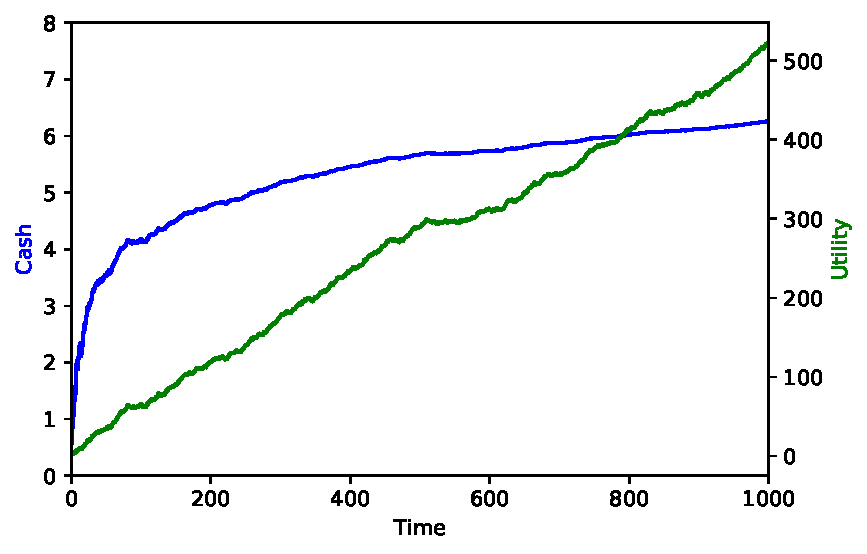
\includegraphics[width=\textwidth]{./chapter_riskless/figs/trajectories.pdf}
%}
%\end{picture}
\caption{\small Typical trajectory $\x(\t)$ of the wealth
dynamic \eref{test_dyn}, with parameter values $\av=1/2$ and $\bv=1$,  and the corresponding Brownian motion $\gv(\t)$. Note that the fluctuations in $\x(\t)$ become smaller for larger wealth. }
\flabel{test_dyn}
\end{figure}

\begin{example}{A curious-looking dynamic}
Given a dynamic, it is possible to check whether an ergodicity mapping exists, 
and the mapping itself can be found. We consider the wealth dynamic
\begin{equation}
\gd\x=\left(\frac{\av}{\bv}e^{-\x}-\frac{1}{2}e^{-2\x}\right)\gd\t+e^{-\x}\gd\gW.
\elabel{test_dyn}
\end{equation}
We note that $\ax(\x)=\frac{\av}{\bv}e^{-\x}-\frac{1}{2}e^{-2\x}$ and $\bx(\x)=e^{-\x}$.
\Eref{consistency} imposes conditions on the drift term $\ax(\x)$ in terms of the 
noise term $\bx(\x)$. Substituting in \eref{consistency} reveals that the consistency 
condition is satisfied by the dynamic in \eref{test_dyn}.
A typical trajectory of \eref{test_dyn} is shown in \fref{test_dyn}.

Because \eref{test_dyn} is internally consistent, it is possible to derive the corresponding utility function.
\Eref{b_u} is a first-order ordinary differential equation for $\gv(\x)$
\begin{align}
\gv'(\x)=\frac{\bv}{\bx(\x)},
\elabel{diff_eq_u}
\end{align}
which can be integrated to
\begin{align}
\gv(\x)=\int_0^\x \gd\tilde{\x} \frac{\bv}{\bx(\tilde{\x})}+C,
\end{align}
with $C$ an arbitrary constant of integration. This constant, incidentally, implies that 
only {\it changes} in utility are meaningful, as was pointed out by von 
Neumann and Morgenstern \cite{vonNeumannMorgenstern1944} -- this robust feature
is visible whether one thinks in dynamic terms, ergodicity mappings, and time averages; 
or in terms of consistent measure-theoretic concepts and expectation values.

Substituting for $\bx(\x)$ from \eref{test_dyn}, \eref{diff_eq_u} becomes
\begin{equation}
\gv'(\x)=\bv e^\x,
\end{equation}
which is easily integrated to
\begin{equation}
\gv(\x)=\bv e^\x +C,
\elabel{test_dyn_u}
\end{equation}
plotted in \fref{u_of_x}. This exponential ergodicity mapping is monotonic and 
therefore invertible -- we knew that because the consistency condition is satisfied. 
The ergodicity mapping is convex. From the 
perspective of expected-utility theory an individual behaving optimally according to 
this function would be labelled ``risk-seeking.'' 
The dynamical perspective corresponds to a qualitatively different interpretation: 
Under the dynamic \eref{test_dyn} the ``risk-seeking'' individual behaves optimally, 
in the sense that his wealth will grow faster than that of a risk-averse individual. 
What's optimal is determined by the dynamic, not by the individual. Of course the 
individual may choose whether to behave optimally. The dynamic \eref{test_dyn} 
has the feature that fluctuations in wealth become smaller as wealth grows. High 
wealth is therefore sticky -- an individual will quickly fluctuate out of 
low wealth and into higher wealth. It will then tend to stay there. 
\end{example}

\begin{figure}
\centering
\begin{picture}(200,80)(0,0)
 \put(-80,0){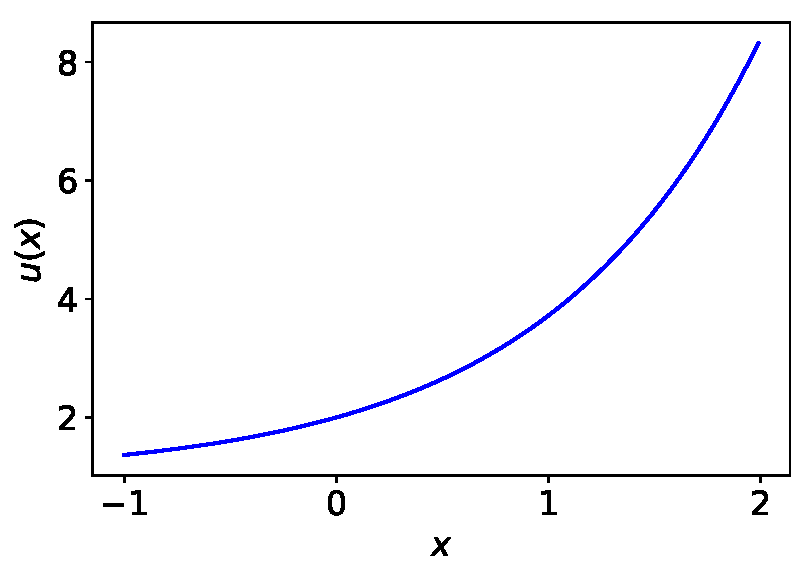
\includegraphics[width=.47\textwidth]{./chapter_riskless/figs/u_of_x.pdf}}
 \put(110,0){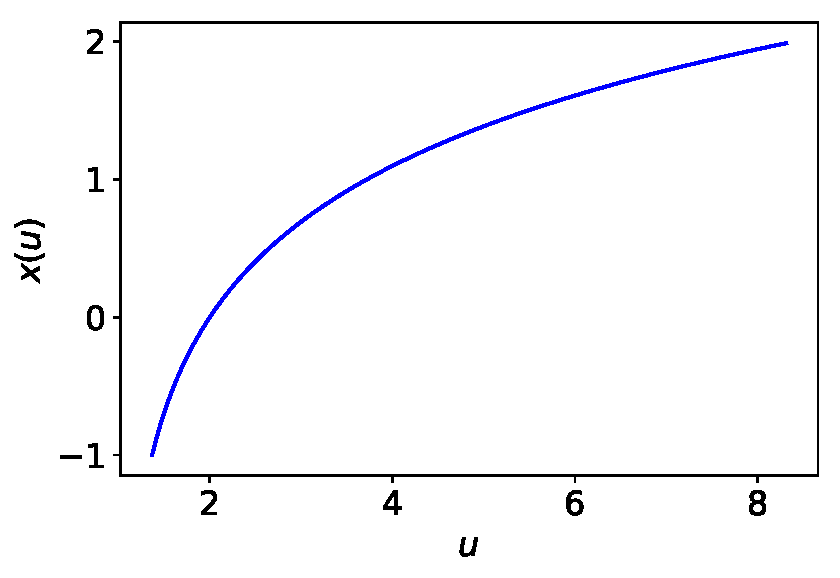
\includegraphics[width=.47\textwidth]{./chapter_riskless/figs/x_of_u.pdf}}
\end{picture}
\caption{\small The exponential ergodicity mapping (or utility) $\gv(\x)$, \eref{test_dyn_u} with $\bv=1$ and $C=1$, is monotonic and unbounded and therefore invertible.
Left panel: $\gv(\x)$. Right panel: inverse $\x(\gv)$.}
\flabel{u_of_x}
\end{figure}


\section{The St Petersburg paradox}
\secref{SPP}
The problem known today as the St Petersburg paradox was suggested by Nicolaus 
Bernoulli\footnote{Daniel's cousin. The Bernoulli family produced a remarkable 
number of famous mathematicians in the $17^\text{th}$ and $18^\text{th}$ centuries, 
who helped lay the foundations of applied mathematics and physics.} in 1713 in his 
correspondence with Montmort~\cite{Montmort1713}. It involves a hypothetical 
lottery for which the rate of change of expected wealth diverges for any finite ticket 
price. The expected-wealth paradigm would predict, therefore, that people are 
prepared to pay any price to enter the lottery. However, when the question is put 
to them, they rarely want to wager more than a few dollars. This 
is the paradox. It is the first well-documented example of the inadequacy of the 
expected-wealth paradigm as a model of human rationality. It was the primary 
motivating example for Daniel Bernoulli's and Cramer's development of the 
expected-utility paradigm~\cite{Bernoulli1738}.

In some sense it is a pity that this deliberately provocative and unrealistic lottery has played such 
an important role in the development of classical decision theory. It is quite unnecessary to invent 
a gamble with a diverging change in expected wealth to expose the flaws in the expected-wealth 
paradigm. The presence of infinities in the problem and its variously proposed solutions has 
caused much confusion, and permits objections on the grounds of physical impossibility. These 
objections don't much advance decision theory: they address only the gamble and 
not the decision paradigm. Nevertheless, the paradox is an indelible part not only of history but 
also of the current debate~\cite{Peters2011b}, and so we recount it here. We'll start by defining 
the lottery.

\begin{example}{St Petersburg lottery}
Imagine a starting prize 
of $\$1$ (originally the prize was in ducats). A fair coin is tossed: 
if it lands heads, the player wins the prize and the lottery ends; if it lands 
tails, the prize is doubled and the process is repeated. Therefore, the 
player wins $\$2$, $\$4$, $\$8$ if the first head lands 
on the second, third, fourth toss, and so on. The player must buy a ticket, 
at price $\F$, to enter the lottery. The question is: what is 
the largest $\F$ the player is willing to pay?

The lottery can be translated neatly into our gamble formalism:
\be
\q_\gj = \$ 2^{\gj-1} - \F, \quad \p_\gj = 2^{-\gj},
\elabel{lottery_def}
\ee
for $\gj\in\{1,2,3,\ldots\}$, \ie the set of positive integers. The vast majority 
of observed payouts are small, but occasionally an extremely large payout 
(corresponding to a very long unbroken sequence of tails in the classical 
description) occurs. This is shown in the example trajectories in 
\fref{lottery_add_traj}, where the lottery has been repeated additively.

From now on we will forget about the coin tosses, which are simply a 
mechanism for selecting one of the possible payouts. They 
are nothing but an 18th-century random number generator. Instead we shall work with the 
compact definition of the lottery in \eref{lottery_def} and assume it 
takes a fixed amount of time, $\dt$, to play.

The rate of change of expected wealth is
\bea
\frac{\ave{\d\x}}{\dt} & = & \frac{1}{\dt} \sum_{\gj=1}^\infty \p_\gj \q_\gj \\
&=& \frac{1}{\dt} \left( \$ \sum_{\gj=1}^\infty 2^{-\gj}\,2^{\gj-1} - \sum_{\gj=1}^\infty 2^{-\gj} \F \right) \\
&=& \frac{1}{\dt} \left( \$ \sum_{\gj=1}^\infty \frac{1}{2} - \F \right). \elabel{lottery_ex_wealth}
\eea
This diverges for any finite ticket price. Under the expected-wealth paradigm, 
this means that the lottery is favourable at any price.
\end{example}
\begin{figure}
\centering
\begin{picture}(200,230)(0,0)
\put(-75,0){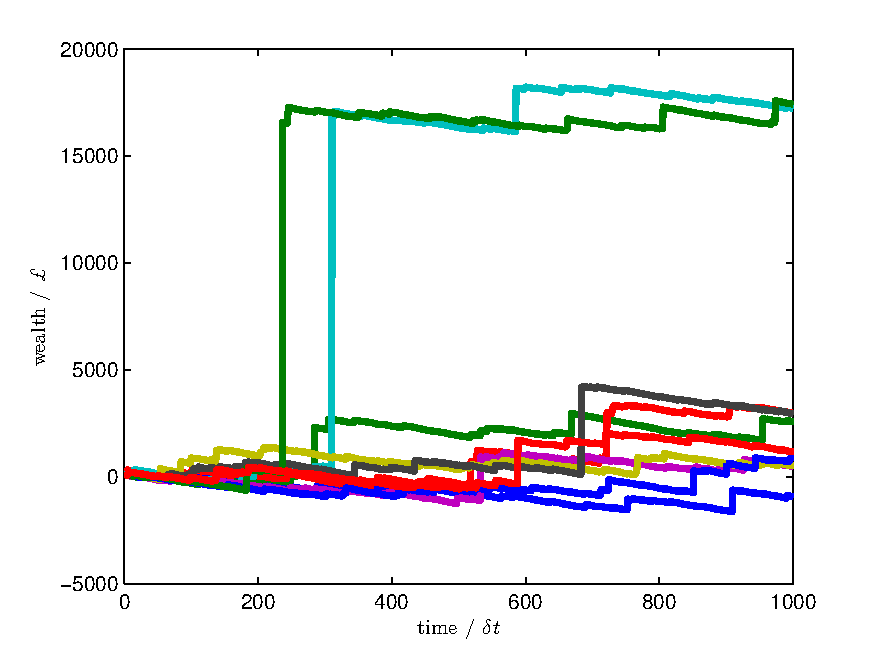
\includegraphics[width=\textwidth]{./chapter_riskless/figs/lottery_add_traj.pdf}}
\end{picture}
\caption{Wealth trajectories for the additively repeated St Petersburg lottery, 
with starting wealth, $\x(0)=\$100$, and ticket price, $\F=\$10$. 
Ten trajectories are plotted over 1,000 rounds.\flabel{lottery_add_traj}}
\end{figure}

This implausible conclusion, which does not accord with human behaviour, 
exposes the weakness of judging a gamble by its effect on expected 
wealth. Daniel Bernoulli suggested to resolve the paradox by adopting 
the expected-utility paradigm. His choice of utility function was the 
logarithm, $\gu(\x)=\ln \x$, which, as we now know, produces a decision 
rule equivalent to growth-rate optimisation under multiplicative repetition. 
This correspondence was not appreciated by Bernoulli: indeed 
$18^\text{th}$-century mathematics did not possess the concepts and 
language required to distinguish between averages over time and across 
systems, even though it had the basic arithmetic tools. 
%In any case, the 
%correspondence relies on the choice of a particular utility function, and vanishes the moment something other than the logarithm is chosen. We also have
%to interpret expected utility theory a little differently from how it is usually presented -- for instance we have to assume that expected changes in utility really mean expected rates of changes, with a specific gamble duration, \ie we have to introduce the concept of time into utility theory quite differently from that's usually done (which we won't discuss here).

Unfortunately, Bernoulli made a mathematical error in the implementation 
of his own paradigm -- accidentally he proposed two mutually inconsistent 
versions of utility theory in the paper that established the paradigm. Initially, 
the error had little impact, and it was corrected by Laplace in 
1814~\cite{Laplace1814}. But Laplace didn't openly say he'd corrected an 
error, he just worked with what he thought Bernoulli had meant. This politeness 
had awful consequences. In 1934 Menger~\cite{Menger1934}, keen to get the 
story right, went back to the original text by Bernoulli. He didn't notice the 
error but rather got confused by it which led him to introduce a further error. 
Based on this car crash of scientific communication, Menger derived the 
infamous (wrong) claim we encountered in the history segment in \secref{dyn_from_u}: utility functions 
must be bounded, with disastrous consequences for the budding neoclassical formalism. We 
will leave this most chequered part of the paradox's history alone -- details can be found 
in~\cite{PetersGell-Mann2016,Peters2019}. Instead we will focus on what's usually 
presumed Bernoulli meant to write.

\begin{example}{Resolution by logarithmic utility}
Instead of \eref{lottery_ex_wealth}, we calculate the rate of change of expected logarithmic utility,
\bea
\frac{\ave{\d\ln \x}}{\dt} & = & \frac{1}{\dt} \sum_{\gj=1}^\infty \p_\gj \left[\ln(\x+\q_\gj)-\ln \x\right] \\
&=& \frac{1}{\dt} \sum_{\gj=1}^\infty 2^{-\gj} \ln\left(\frac{\x+\$2^{\gj-1}-\F}{\x}\right), \elabel{lottery_ex_util}
\eea
where $\x$ is the ticket buyer's wealth.

This is finite for all finite ticket prices less than the buyer's wealth plus the smallest 
prize: $\F<\x+\$1$. This can be shown by applying the ratio 
test.\footnotemark\ It may be positive or negative, depending on the values 
of $\F$ and $\x$. \fref{gbar_zero} shows the locus of points in the $(\x,\F)$-plane 
for which the sum is zero.
\end{example}
\footnotetext{The ratio of the $(\gj+1)^\text{th}$ term to the $\gj^\text{th}$ term 
in the sum tends to $1/2$ as $\gj\to\infty$.}
\begin{figure}
\centering
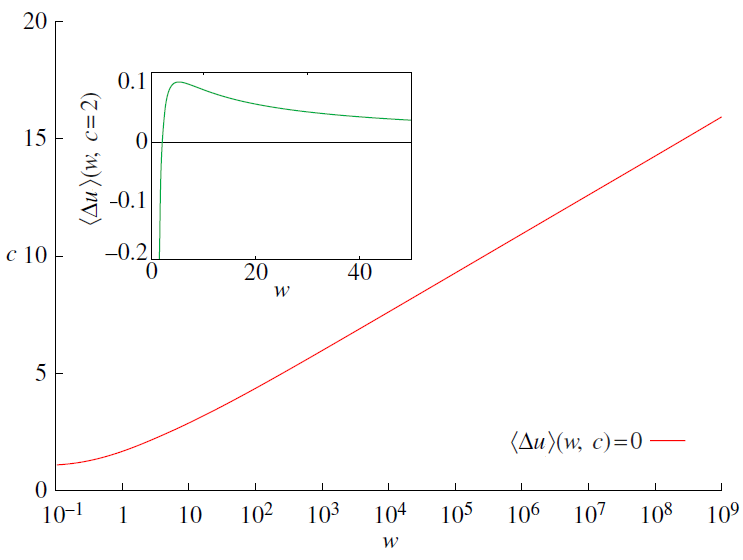
\includegraphics[width=\textwidth]{./chapter_riskless/figs/gbar_zero.png}
\caption{Locus of points in the $(\x,\F)$-plane for which the expected change in 
logarithmic utility is zero. The inset shows the expected change in utility as a 
function of $\x$ for $\F=\$2$. Adapted from~\cite{Peters2011b}.\flabel{gbar_zero}}
\end{figure}

The utility paradigm is a model that resolves the paradox, in the sense that creates 
a world where players may decline to buy a ticket. Bernoulli argued for this resolution 
framework in plausible terms: the usefulness of a monetary gain depends on how 
much money you already have. He also argued specifically for the logarithm in 
plausible terms: the gain in usefulness should be proportional to the fractional gain 
it represents, $\d \gu = \d\x/\x$. Yet, the framework has left many unsatisfied: why 
does usefulness have this functional form? We provide this deeper reason by 
connecting the problem to dynamics and time, unlike Bernoulli. Had Bernoulli made 
the connection, he might have been less willing to accept Cramer's square-root utility 
function as an alternative, which, as we've seen, corresponds to a rather less intuitive dynamic.

%However, while plausible, the framework relies on a utility function, which must be postulated. It can neither be derived from fundamental considerations nor verified empirically.

Turning to our decision algorithm, we will assume that the lottery is assessed by
the growth rate it would impart on the player were it repeated 
multiplicatively. This means, in effect, that the prizes and ticket price are treated 
as fractions of the player's wealth, such that the effect of each lottery is to 
multiply current wealth by a random factor,
\be
\gr_\gj = \frac{\x+\$2^{\gj-1}-\F}{\x}, \quad \p_\gj= 2^{-\gj}.
\ee
This follows precisely our earlier treatment of a gamble with multiplicative dynamics, 
and we can apply our results directly. The time-average (exponential) growth rate is
\be
\gt_\text{m} = \frac{1}{\dt} \lim_{\T\to\infty} \left\{ \frac{1}{\T}  \sum_{\gtau=1}^\T \ln \gr(\gtau) \right\} = \frac{1}{\dt}  \sum_{\gj=1}^\infty 2^{-\gj} \ln \gr_\gj, \elabel{lottery_gbar}
\ee
which is identical to the expression for the rate of change of expected log-utility, 
\eref{lottery_ex_util}. This is, as we've discussed, because $\gv(\x)=\ln(\x)$ 
is the appropriate ergodicity mapping for multiplicative dynamics. The result is the same, but 
the interpretation is different: we have assumed less, only that our player is 
interested in the growth rate of his wealth and that he gauges this by imagining 
the outcome of an indefinite sequence of repeated lotteries.

Thus the locus in \fref{gbar_zero} also marks the decision threshold \textit{versus} 
the null gamble under our decision axiom. The player can sensibly decline the 
gamble, even though it results in a divergent change in expected wealth. This 
is illustrated by comparing \fref{lottery_mult_traj}, which shows trajectories of 
multiplicatively repeated lotteries, with the additively repeated lotteries already 
seen in \fref{lottery_add_traj}.
\begin{figure}
\centering
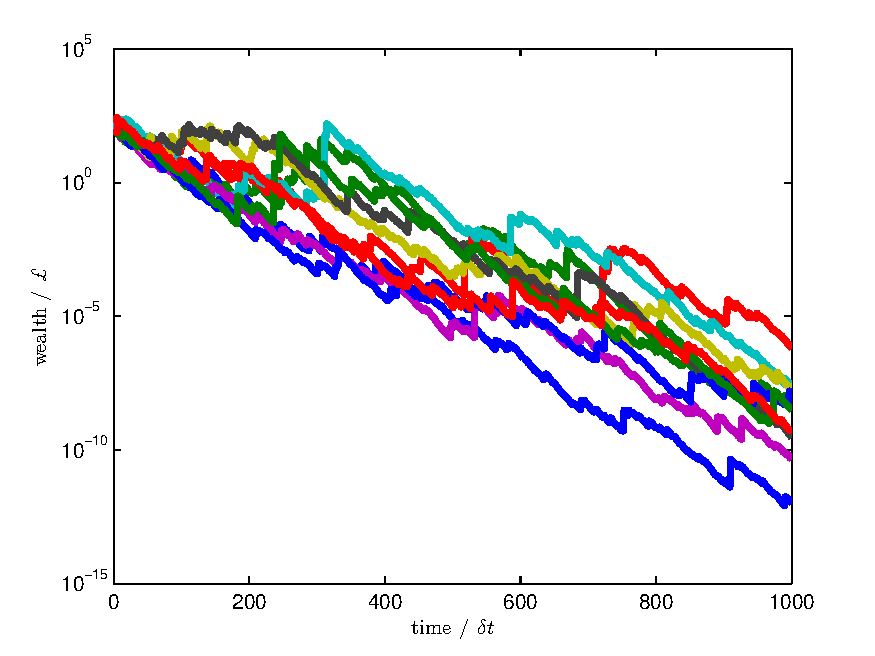
\includegraphics[width=\textwidth]{./chapter_riskless/figs/lottery_mult_traj.pdf}
\caption{Wealth trajectories for the multiplicatively repeated St Petersburg lottery, 
with starting wealth, $\x(0)=\$100$, and ticket price, $\F=\$10$. Ten 
trajectories are plotted over 1,000 rounds. The realisations of the individual 
lotteries are the same as in \fref{lottery_add_traj} but the mode of repetition is 
different.\flabel{lottery_mult_traj}}
\end{figure}
The trajectories are based on the same sequences of lottery outcomes, only 
the mode of repetition is different. The simulation shows us visually what we 
have already gleaned by analysis: what appears favourable in the 
expected-wealth paradigm (corresponding to additive repetition) results in a 
disastrous decay of the player's wealth over time under a realistic dynamic.

As $\F\to \x+\$1$ from above in \eref{lottery_gbar}, $\gt_\text{m}$ diverges 
negatively, since the first term in the sum is the logarithm of a quantity approaching 
zero. This corresponds to a lottery which can make the player bankrupt. The effect 
is also shown in the inset of \fref{gbar_zero}.

Treatments based on multiplicative repetition have appeared sporadically in the 
literature, starting with Whitworth in 
1870~\cite[App.~IV]{Whitworth1870}.\footnote{Whitworth was dismissive of early 
utility theory: ``The result at which we have arrived is not to be classed with 
the arbitrary methods which have been again and again propounded to evade 
the difficulty of the Petersburg problem\ldots. Formulae have often been proposed, 
which have possessed the one virtue of presenting a finite result\ldots but they 
have often had no intelligible basis to rest upon, or\ldots sufficient care has not 
been taken to draw a distinguishing line between the significance of the result 
obtained, and the different result arrived at when the mathematical expectation 
is calculated.'' Sadly he chose to place these revolutionary remarks in an appendix 
of a college probability textbook.} It is related to the famous Kelly 
Criterion~\cite{Kelly1956}\footnote{Kelly was similarly unimpressed with the 
mainstream and noted in his treatment of decision theory, which he developed 
from the perspective of information theory and which is identical to ergodicity 
economics with multiplicative dynamics, that the utility function is ``too general 
to shed any light on the specific problems of communication theory.''}, although 
Kelly did not explicitly treat the St Petersburg game, and tangentially to \Ito's 
lemma~\cite{Ito1944}. It appears as an exercise in a well-known text on information 
theory~\cite[Ex.~6.17]{CoverThomas1991}. Mainstream economics has ignored all 
this. A full and rigorous resolution of the paradox, including the epistemological 
significance of the shift from ensemble to time averages, was published recently 
by one of the present authors~\cite{Peters2011b}.
